%%%%%%%%%%%%%%%%%%%%%%%%%%%%%%%%%%%%%%%%%%%%%%%%%%%%%%%%%%%%
%%% ELIFE ARTICLE TEMPLATE
%%%%%%%%%%%%%%%%%%%%%%%%%%%%%%%%%%%%%%%%%%%%%%%%%%%%%%%%%%%%
%%% PREAMBLE 
\documentclass[11pt,onehalfspacing]{elife}
% Use the onehalfspacing option for 1.5 line spacing
% Use the doublespacing option for 2.0 line spacing
% Please note that these options may affect formatting.
% Additionally, the use of the \newcommand function should be limited.


%\usepackage{lipsum} % Required to insert dummy text
\usepackage[version=4]{mhchem}
\usepackage{siunitx}
\usepackage{graphicx}
%\usepackage[unicode]{hyperref}
\usepackage{listings}
\lstset{frame=none,
  language=R,
  aboveskip=3mm,
  belowskip=3mm,
  showstringspaces=false,
  columns=flexible,
  basicstyle={\small\ttfamily},
  numbers=none,
  numberstyle=\small\color{black},
  keywordstyle=\color{black},
  commentstyle=\color{black},
  stringstyle=\color{black},
  breaklines=true,
  breakatwhitespace=true,
  tabsize=3
}
\DeclareSIUnit\Molar{M}


%%%%%%%%%%%%%%%%%%%%%%%%%%%%%%%%%%%%%%%%%%%%%%%%%%%%%%%%%%%%
%%% ARTICLE SETUP
%%%%%%%%%%%%%%%%%%%%%%%%%%%%%%%%%%%%%%%%%%%%%%%%%%%%%%%%%%%%
\title{
Tehnici de monitorizare a deplasărilor animalelor sălbatice}

% \presentadd[\authfn{5}]{eLife Sciences editorial Office, eLife Sciences, Cambridge, United Kingdom}

%%%%%%%%%%%%%%%%%%%%%%%%%%%%%%%%%%%%%%%%%%%%%%%%%%%%%%%%%%%%
%%% ARTICLE START
%%%%%%%%%%%%%%%%%%%%%%%%%%%%%%%%%%%%%%%%%%%%%%%%%%%%%%%%%%%%
\begin{document}
\begin{titlepage}

\newcommand{\HRule}{\rule{\linewidth}{0.2mm}}     
      
\begin{figure}[t]
\begin{minipage}{0.6\textwidth}\large
\begin{flushleft}

\includegraphics[width=0.8\textwidth]{UB.jpg}
\end{flushleft}
\end{minipage}
\begin{minipage}{0.4\textwidth}\large
\begin{flushright}

\includegraphics[width=1\textwidth]{logo-multidimension.png}

\end{flushright}
\end{minipage}
\end{figure}
\textsc{ \\[1cm]}


\begin{center}
\HRule
\\[0.5cm]
\textbf{\Large   Tehnici de monitorizare a deplasărilor animalelor sălbatice}
\HRule
\\[0.5cm]
\textbf{\large Manual}
\\[0.25cm]
\large      
{Laurentiu Rozylowicz | Florian P. Bodescu |  Athanasios A. Gavrilidis | Iulia V. Miu | Cristian Moale | Steluta Manolache | Andreea Nita | Marius L. Matache |\\ Cristiana M. Ciocanea}
   \end{center}
        
\vfill 
  \begin{center}
    \textbf{\large      
Universitatea din București | Multidimension R\&D\\[0.25cm]
proiect PN-III-P2-2.1-PED-2016-0568 - Argos based applications for real time wildlife monitoring in Romania (BioMoveFix), finanțat de UEFISCDI}\\
        \end{center}
\vfill 

\begin{center}
\textbf{București 2018}\\
\url{https://github.com/rlaurentiu/BioMoveFix}
 \end{center}
        
\end{titlepage}
\newpage
\begin{titlepage}
~\vfill
\setlength{\parindent}{0pt}
\setlength{\parskip}{\baselineskip}

\par {Manual publicat de Universitatea din București, Centrul de Cercetare a Mediului și Efectuare a Studiilor de Impact}

\par {Rozylowicz, L., Bodescu, F. P., Gavrilidis, A. A., Miu, I. V., Moale, C., Manolache, S., Nita, A., Matache, M. L., Ciocanea, C. M. (2018). Tehnici de monitorizare a deplasărilor animalelor sălbatice. Manual. București: Universitatea din București. Centrul de Cercetare a Mediului și Efectuare a Studiilor de Impact. Biodiversity Literature Repository. doi:10.5281/zenodo.1344840}

\par{resurse suplimentare: \url{https://github.com/rlaurentiu/BioMoveFix}}

\par{\url{www.ccmesi.ro} | \url{www.multidimension.ro}}\\

\par{Acest manual este produs în cadrul proiectului PN-III-P2-2.1-PED-2016-0568 "Argos based applications for real time wildlife monitoring in Romania (BioMoveFix)", finanțat de Unitatea Executivă pentru Finanțarea Învățământului Superior, a Cercetării, Dezvoltării și Inovării (UEFISCDI) prin programul PNCDI III - P2 - Creșterea competitivității economiei românești prin CDI, Proiect experimental demonstrativ (PED)}\\

Copyright \copyright\ \the\year~Universitatea din București \& Multidimension SRL\\

\par This work is licensed under the Creative Commons Attribution-NonCommercial 4.0 International License. To view a copy of this license, visit \url{https//creativecommons.org/licenses/by-nc/4.0/} or send a letter to Creative Commons, PO Box 1866, Mountain View, CA 94042, USA.\index{license}

\par\text{Bucuresti, mai, 2018}
\clearpage
\end{titlepage}

\tableofcontents
\clearpage
\section{Obiectivele monitorizării în timp real a deplasărilor animalelor sălbatice}

Tehnologiile moderne pentru monitorizarea de la distanță a speciilor de animale sălbatice permit cercetătorilor să răspundă la câteva probleme fundamentale de ecologie cum ar fi utilizarea habitatelor, selecția resurselor și migrații \citep{wilmers_nickel_bryce_smith_wheat_yovovich_2015}. Studiul deplasării animalelor permite abordarea mai multor obiective de cercetare specifice ecologiei, cele mai comune fiind analiza dinamicii populațiilor, analiza distribuției spațiale a indivizilor și populațiilor, analiza home-range-ului, migrațiilor și deplasărilor locale, studiul dispersiei și analiza memoriei spațiale a indivizilor și populațiilor \citep{Hooten2017}.

\textbf{Dinamica populațiilor} reprezintă o informație cheie pentru determinarea gradului de vulnerabilitate a unei specii sau populații dintr-un anumit spațiu geografic \citep{Hooten2017}. Aceasta poate fi estimată prin  integrarea datelor de natalitate, mortalitate și emigrare \citep{begon_harper_townsend_2006}. Acești parametrii pot fi determinați cu ajutorul telemetriei, prin extrapolarea datelor provenite de la indivizii studiați. Telemetria oferă informații la o scară temporală redusă și poate evidenția existența unei perturbări apărută relativ spontan. Odată identificată problema se creează cadrul necesar investigării aprofundate a cauzelor care au condus la generarea ei \citep{gaillard_festa-bianchet_yoccoz_1998, bowler_benton_2005}.

\textbf{Analiza distribuției spațiale a populațiilor} reprezintă un alt obiectiv care poate fi abordat cu ajutorul telemetriei, prin determinarea indirectă a densității populației și analiza deplasărilor indivizilor într-un areal \citep{Hooten2017}. Expansiunea teritorială a unei specii poate fi legată de o serie de factori precum lipsa prădătorilor sau abundența de resurse care permit creșterea densității populației \citep{blondel_chessel_frochot_1988, mitani_watts_amsler_2010, christensen_radford_2018}. Pe de altă parte, scăderea densității populației dintr-un spațiu poate semnala o degradare a habitatelor sau o mortalitate ridicată. Tehnicile de monitorizare actuale au capacitatea de a furniza informații cu privire la distribuția spațială a indivizilor, facilitând demararea investigațiilor ulterioare legate de amenințări existente și planificarea conservării \citep{guisan_thuiller_2005}.

Unele obiectivele majore ale analizei mișcării indivizilor sunt legate de obținerea datelor despre \textbf{home range, areal de distribuție și concentrarea indivizilor} \citep{Hooten2017}. Fidelitatea unor specii față de un teritoriu poate fi explicată în diverse moduri, dintre care amintim prezența surselor de hrană, favorabilitatea pentru activitățile de reproducere sau lipsa amenințărilor externe \citep{schjorring_gregersen_bregnballe_2000}. Aceste areale pot fi perturbate de indivizi ai aceleiași specii (în cazul speciilor teritoriale) care pot intra în competiție cu populația locală sau de factori externi (antropici sau naturali, inclusiv alte specii) \citep{frid_dill_2002}. Astfel, mijloacele de monitorizare moderne pot facilita analiza acestor modele comportamentale prin identificarea modului în care indivizii accesează, utilizează sau se deplasează într-un teritoriu. Prin telemetrie se poate identifica și modul în care indivizi din cadrul aceleași specii interacționează în cadrul unui teritoriu \citep{millspaugh_2001}.

\textbf{Mișcările de grup (e.g., migrațiile)} și \textbf{deplasările locale} ale indivizilor reprezintă informații cheie în conservarea biodiversității, în special pentru planificarea conservării și combaterea braconajului \citep{Hooten2017}. S-a demonstrat faptul că măsurile de conservare  aplicate în teritoriile „destinație” ale speciilor migratoare sunt ineficiente dacă acestea nu sunt completate cu măsuri specifice pe rutele de migrațiune sau în teritoriile de odihnă \citep{singh_milner-gulland_2010}. Utilizarea mijloacelor de monitorizare prin telemetrie are ca obiectiv principal identificarea rutelor de deplasare ale grupurilor de indivizi. Datele furnizate în urma acestui tip de analize reprezintă informații vitale în procesul de luare a deciziei cu privire la conservare \citep{martell_henny_nye_solensky_2001, hebblewhite_haydon_2010}.

\textbf{Dispersia indivizilor} unei specii este un alt obiectiv major al studiilor de mișcare a animalelor \citep{Hooten2017}. S-a demonstrat că indivizii sunt atrași de arealele în au condiții reproductive mai bune și acces la hrană mai facil \citep{begon_harper_townsend_2006}. Astfel de informații pot fi transmise între indivizi din grupuri și teritorii diferite care ajung să interacționeze. În final, indivizii din habitate cu condiții precare sunt atrași în teritoriile mai bune \citep{Hooten2017}.

Un obiectiv mai actual al utilizării tehnicilor de monitorizare de la distanță îl reprezintă studierea \textbf{memoriei spațiale a indivizilor sau populațiilor} \citep{Hooten2017}. De exemplu, monitorizarea unui individ pe parcursul a 5 ani poate furniza informații referitoare la modul în care acesta se comportă în raport cu teritoriile pe care le accesează. Dacă acesta își schimbă ruta de migrație sau zona de cuibărit în funcție de resursele nou descoperite, atunci se pot deduce concluzii pertinente cu privire la modul în care indivizii unei specii fac apel la memoria spațială pentru selectarea habitatelor propice, dând posibilitatea cercetătorilor de a crea modele comportamentale specifice.

Conexiunile dintre \textbf{condiția fiziologică a individului, modul de deplasare și teritoriu} este alt obiectiv ce poate fi abordat prin telemetrie. În trecut, astfel de studii complexe presupuneau recapturarea individului pentru efectuarea unor analize morfologice și fiziologice \citep{Hooten2017}, dar dezvoltarea biotelemetriei facilitează observarea de la distanță a unor aspecte fiziologice ale individului monitorizat (e.g., puls, temperatura corpului, creștere) care pot fi apoi corelate cu accesarea anumitor teritorii \citep{wilmers_nickel_bryce_smith_wheat_yovovich_2015}. Astfel, se poate face saltul la un nou obiectiv al monitorizării animalelor sălbatice și anume acela de \textbf{evaluare a balanței energetice a indivizilor} \citep{Hooten2017}. 


\section{Tehnologii de monitorizare}
\subsection{Radiotelemetrie prin unde de frecvență foarte înaltă (VHF)}
Monitorizarea animalelor sălbatice cu ajutorul transmițătoarelor de unde radio de frecvență foarte înaltă constituie cea mai veche tehnică de înregistrare a poziției unui individ în mediul natural de la distanță \citep{White2012}. Poziția individului nu este înregistrată automat ci necesită localizarea activă de către cercetător cu ajutorul unei antene direcționale (Yagi) și a unui receptor radio \citep{Silvy2012}. Sistemul de radiotelemetrie VHF trebuie să includă: emițător radio atașat de individul monitorizat, receptor radio VHF, antena Yagi (Figura ~\ref{fig1}).
\begin{figure}[ht]
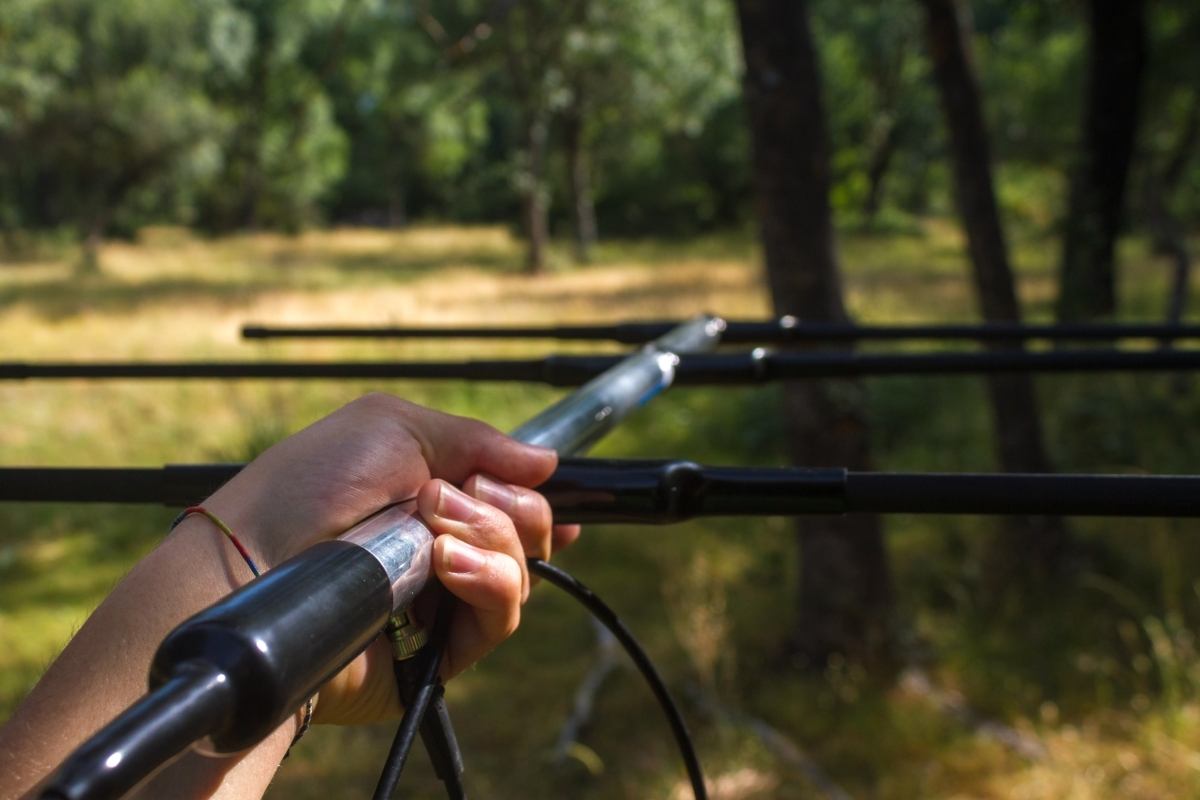
\includegraphics[width=\textwidth]{Fig1.jpg}
\caption{Antena Yagi portabilă pentru recepție semnal VHF (© Shutterstock).} \label{fig1}
\end{figure}

Emițătorul radio poate cântări de la sub un gram la peste un kilogram. Dimensiunile depind de durata de viață a emițătorului și tipul de atașare pe animal (e.g., implant, guler, crotal, rucsac, lipit, atașat de pene, membre sau coadă). Emițătorul radio transmite un semnal radio de înaltă frecvență pe o lungime de undă unică pentru fiecare animal monitorizat (e.g., 150 MHz, cu alocări de frecvență pentru fiecare individ din circa 20 în 20 KHz) \citep{White2012}. Lungimea de undă alocată trebuie să fie cât mai aproape de 150 MHz din considerente de mărime a antenei, pentru alte frecvențe fiind necesare antene mari, neportabile. Cu cât durata de viață a emițătorului este mai mare, cu atât dimensiunile lui sunt mai mari \citep{Thomas2012}. Pentru speciile care pot fi recapturate fără efort mare (e.g., țestoase terestre) se poate opta pentru modele cărora li se pot schimba bateriile în teren. Unele emițătoare au microcontrolere care opresc transmisia în anumite perioade din zi, an etc. și controlează durata transmisiei (e.g., puls de 20 milisecunde la fiecare secundă). Microcontrolerul poate schimba și durata pulsului atunci când transmițătorul nu se mișcă pe o perioadă de timp predeterminată și se activează senzorul de mortalitate \citep{Silvy2012}. În vederea obținerii unor date de calitate, la alegerea emițătorului este vitală consultarea producătorului asupra caracteristicilor finale, care trebuie să fie adaptate mediului și speciei de interes (de exemplu, nu se activează senzorul de mortalitate la speciile care stau o perioadă mare în vizuină).

Receptorul radio și antena Yagi sunt special construite pentru frecvențele emițătoarelor și sunt indispensabile pentru localizarea indivizilor. Cu receptorul radio fixat pe frecvența de interes se înregistrează coordonatele poziției din care se face înregistrarea și azimutul direcției unde semnalul recepționat este cel mai puternic. Pentru o localizare validă trebuie efectuate cel puțin 3 măsurători din 3 poziții diferite \citep{White2012}. Localizarea este calculată manual pe hartă sau într-o aplicație dedicată prin triangulație. Azimuturile pentru o localizare trebuie luate în timp relativ scurt (maxim câteva ore). Acuratețea localizării este variabilă deoarece semnalul poate fi reflectat de elemente din mediu, cum ar fi versanți \citep{Boitani2000}. Precizia localizării este în general de circa 200-600 m atunci când cercetătorul care triangulează este experimentat \citep{Silvy2012}.

Localizarea prin radiotelemetrie VHF se poate face pe jos, din mașină, din avion ușor sau dintr-un turn de recepție. Localizarea se mai poate face și prin urmărirea intensității semnalului până la contactul vizual cu individul care are montat emițător radio \citep{Silvy2012} (homing, vezi demonstrarea metodei la țestoasa lui Hermann, \url{https://www.youtube.com/watch?v=fdZV7kDmfRQ})

Cu toate că prețurile dispozitivelor de monitorizare sunt mici, costurile finale ale cercetării sunt ridicate, deoarece activitatea de monitorizare necesită prezență în teren pentru fiecare triangulație. Astfel, costurile includ și salariul echipelor de radiotelemetrie pe perioada monitorizării, transport și cazare. Numărul de localizări obținute pentru un individ este de regulă mic, mai ales la speciile foarte mobile. De altfel, aceste studii sunt recomandate doar pentru specii care au deplasări mici deoarece semnalul este recepționat până la 5km în condiții de recepție bune \citep{Silvy2012}.

\subsection{Localizare GPS}
Dispozitivele de navigare prin sateliți (GNSS-Global Navigation Satellite System) localizează indivizii monitorizați prin conectarea la una din cele trei rețele globale de poziționare: GPS (rețeaua SUA, cea mai dezvoltată), GLONASS (rețeaua Federației Ruse), Galileo (rețeaua Uniunii Europene) \citep{Madry2015}. Dispozitivele de navigare montate pe animale sunt vizibile în orice moment pentru cel puțin 4 sateliți din constelația GPS. Fiecare satelit vizibil receptorului GPS transmite către acesta mesaje conținând poziția satelitului și timpul înregistrării poziției, cu care receptorul își calculează poziția (Figura ~\ref{gps}). Precizia estimării depinde de numărul de sateliți vizibili și de caracteristicile mediului, dar în general este sub 10m \citep{Silvy2012, Madry2015}.

\begin{figure}[ht]
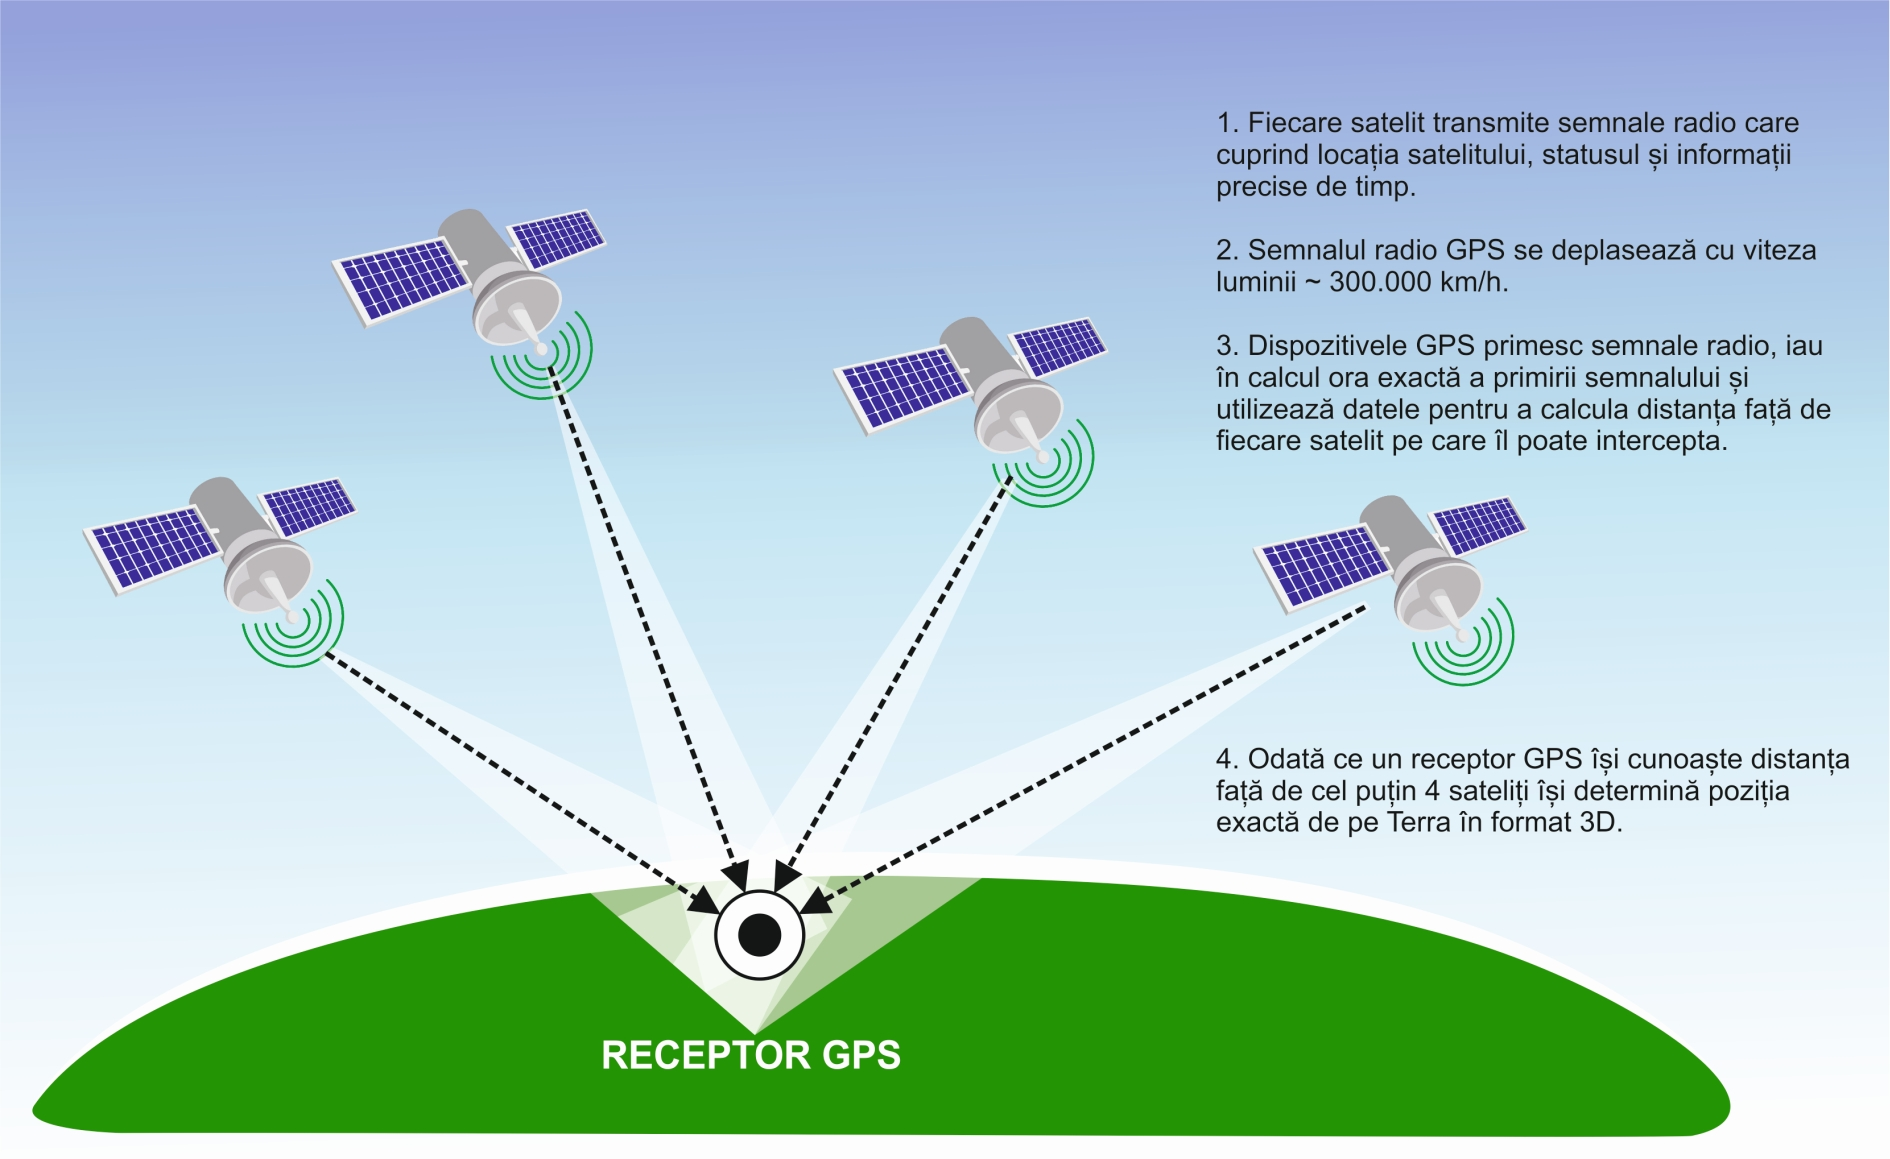
\includegraphics[width=\textwidth]{gps.jpg}
\caption{Localizarea cu ajutorul sistemelor GPS \citep{Madry2015}} \label{gps}
\end{figure}

Sursa de energie, care crește greutatea acestor dispozitive, este o baterie cu litiu, permanentă sau detașabilă, sau un panou solar și o baterie mică de avarie pentru păstrarea datelor stocate în memoria internă. Greutatea este variabilă, de la câteva grame pentru dispozitive care iau câteva poziții (PinPoint GPS) la câteva sute de grame (GPS Iridium). Receptoarele pot fi de tip colier, guler, crotal, atașat de membre, lipite pe carapacea sau pielea mamiferelor marine sau a peștilor de dimensiuni mai mari \citep{Thomas2012}.

Frecvența cu care sunt înregistrate pozițiile indivizilor, depinde de setările dispozitivului de navigare. Odată cu creșterea frecvenței localizărilor cresc și necesitățile de energie și deci mărimea dispozitivului. 

După modul de recuperare a datelor, dispozitivele GPS pot fi \citep{Thomas2012}:

\begin{itemize}
  \item \textbf{GPS store on board.} GPS cu date stocate permanent în memoria internă. Acest tip necesită recapturarea animalului în vederea recuperării datelor sau au un sistem drop-off care se activează la o anumită dată sau la consumarea energiei.\\
  \item \textbf{GPS VFH/UHF.} Datele sunt stocate în memoria on board pentru o perioadă de timp și transmise prin unde radio (UHF, VHF) atunci când cercetătorul se apropie de animal și comandă activarea transmițătorului radio, similar sistemului wireless. Mai rar se întâlnesc și versiuni cu Bluetooth. Acest tip necesită receptor UHF/VHF cu capacitate de recepție și stocare de date și antenă.\\
  \item \textbf{GPS Iridium/Globalstar/Argos.} Datele sunt stocate în memoria on board și transmise prin uplink către o constelație de sateliți predefinită (Iridium/Globalstar/Argos) și apoi utilizatorului. Acest tip necesită plata recepției datelor și a unui abonament lunar.\\
  \item \textbf{GPS GSM.} Datele sunt stocate în memoria on board și transmise prin uplink către rețeaua GSM/GPRS atunci când intră în aria de recepție a unui turn GSM. Necesită cartelă SIM activă și plata abonamentului pentru date mobile. Se poate configura și pentru transmisie GSM/GPRS către sateliți geostaționari (pentru zonele cu acoperire GSM/GPRS slabă).
\end{itemize}

Un sistem experimental care va fi disponibil în anii următori este ICARUS. Acesta va permite construirea unui GPS utilizabil pentru o perioadă mai lungă de timp, având totodată o greutate mică, de circa 5g \citep{Bridge2011}. Sistemul va permite localizare GPS dar și achiziția de alte date prin senzori precum temperatură, accelerometru 3D, magnetometru. Greutatea mai mică va fi posibilă datorită faptului că datele vor fi transmise către senzorii ICARUS de pe International Space Station (ISS) care este mai aproape de Terra. Ulterior testării pe ISS, sistemul se poate muta pe sateliți cu orbită joasă (\url{https://icarusinitiative.org}).

Dispozitivele GPS pot fi echipate cu microcontrolere ON/OFF (pentru activarea la o anumită perioadă), senzor drop-off (mai ales pentru cele tip colier), panou solar, transmițător VHF/UHF pentru senzor de mortalitate și localizare în teren inclusiv după drop-off, senzori cum ar fi accelerometru, temperatură, lumină etc. \citep{Madry2015}.

Costurile echipamentelor GPS sunt ridicate dar monitorizarea nu necesită prezență permanentă în teren. Numărul de localizări precise este de regulă mare. Sistemele cu uplink prin satelit se pretează pentru studiul animalelor care se deplasează mult.

\subsection{Localizare Doppler Argos}
Dacă sistemul GPS utilizează poziția sateliților din constelațiile GPS, GLONASS sau Galileo pentru a calcula poziția în interiorul receptorului, localizarea Doppler Argos (Advanced Research and Global Observation Satellite) utilizează variația frecvenței sunetului emis de receptor la diferite momente pentru a calcula poziția într-un centru de date \citep{Thomas2012}. Platforma Argos (Platform Transmitter Terminal sau PTT) este un dispozitiv care are încorporat un transmițător radio pe o frecvență unică. Frecvența PTT-urilor este în banda de 401.650 MHz ± 30 kHz și este înregistrată în centrul de date Argos ca identificator unic al platformei. Fiecare platformă transmite semnalul radio la intervale de 90-200 secunde, în funcție de setările inițiale în formă de mesaj. Mesajul conține id-ul platformei, data acestuia și informații obținute de la senzorii încorporați (temperatură, lumină, accelerometru etc.).

Semnalul codat este transmis către unul din cei 6 sateliți care au instrumente Argos (SARAL, METOP-B, NOAA-N', METOP-A, NOAA-18, NOAA-15), unde se adaugă frecvența mesajului, poziția satelitului și data recepției, fiind apoi retransmis către centrul de procesare date (de exemplu, CLS). O localizare geografică este stabilită din cel puțin 1 mesaj, dar cu cât sunt mai multe mesaje pentru o localizare, cu atât aceasta este mai precisă \citep{CLS2016}. În principiu, fiecare dintre cei 6 sateliți sunt vizibili de circa 14 ori pe zi din orice zonă de pe Terra, iar fereastra de vizibilitate este de aproximativ 10 minute pentru 1 PTT. Sateliții au instrumente Argos din generațiile 2 sau 3, astfel că mesajele venite de la sateliții cu instrumente din generația 3 sunt mai precise (Figura ~\ref{fig2}) \citep{CLS2016}.

\begin{figure}[ht]
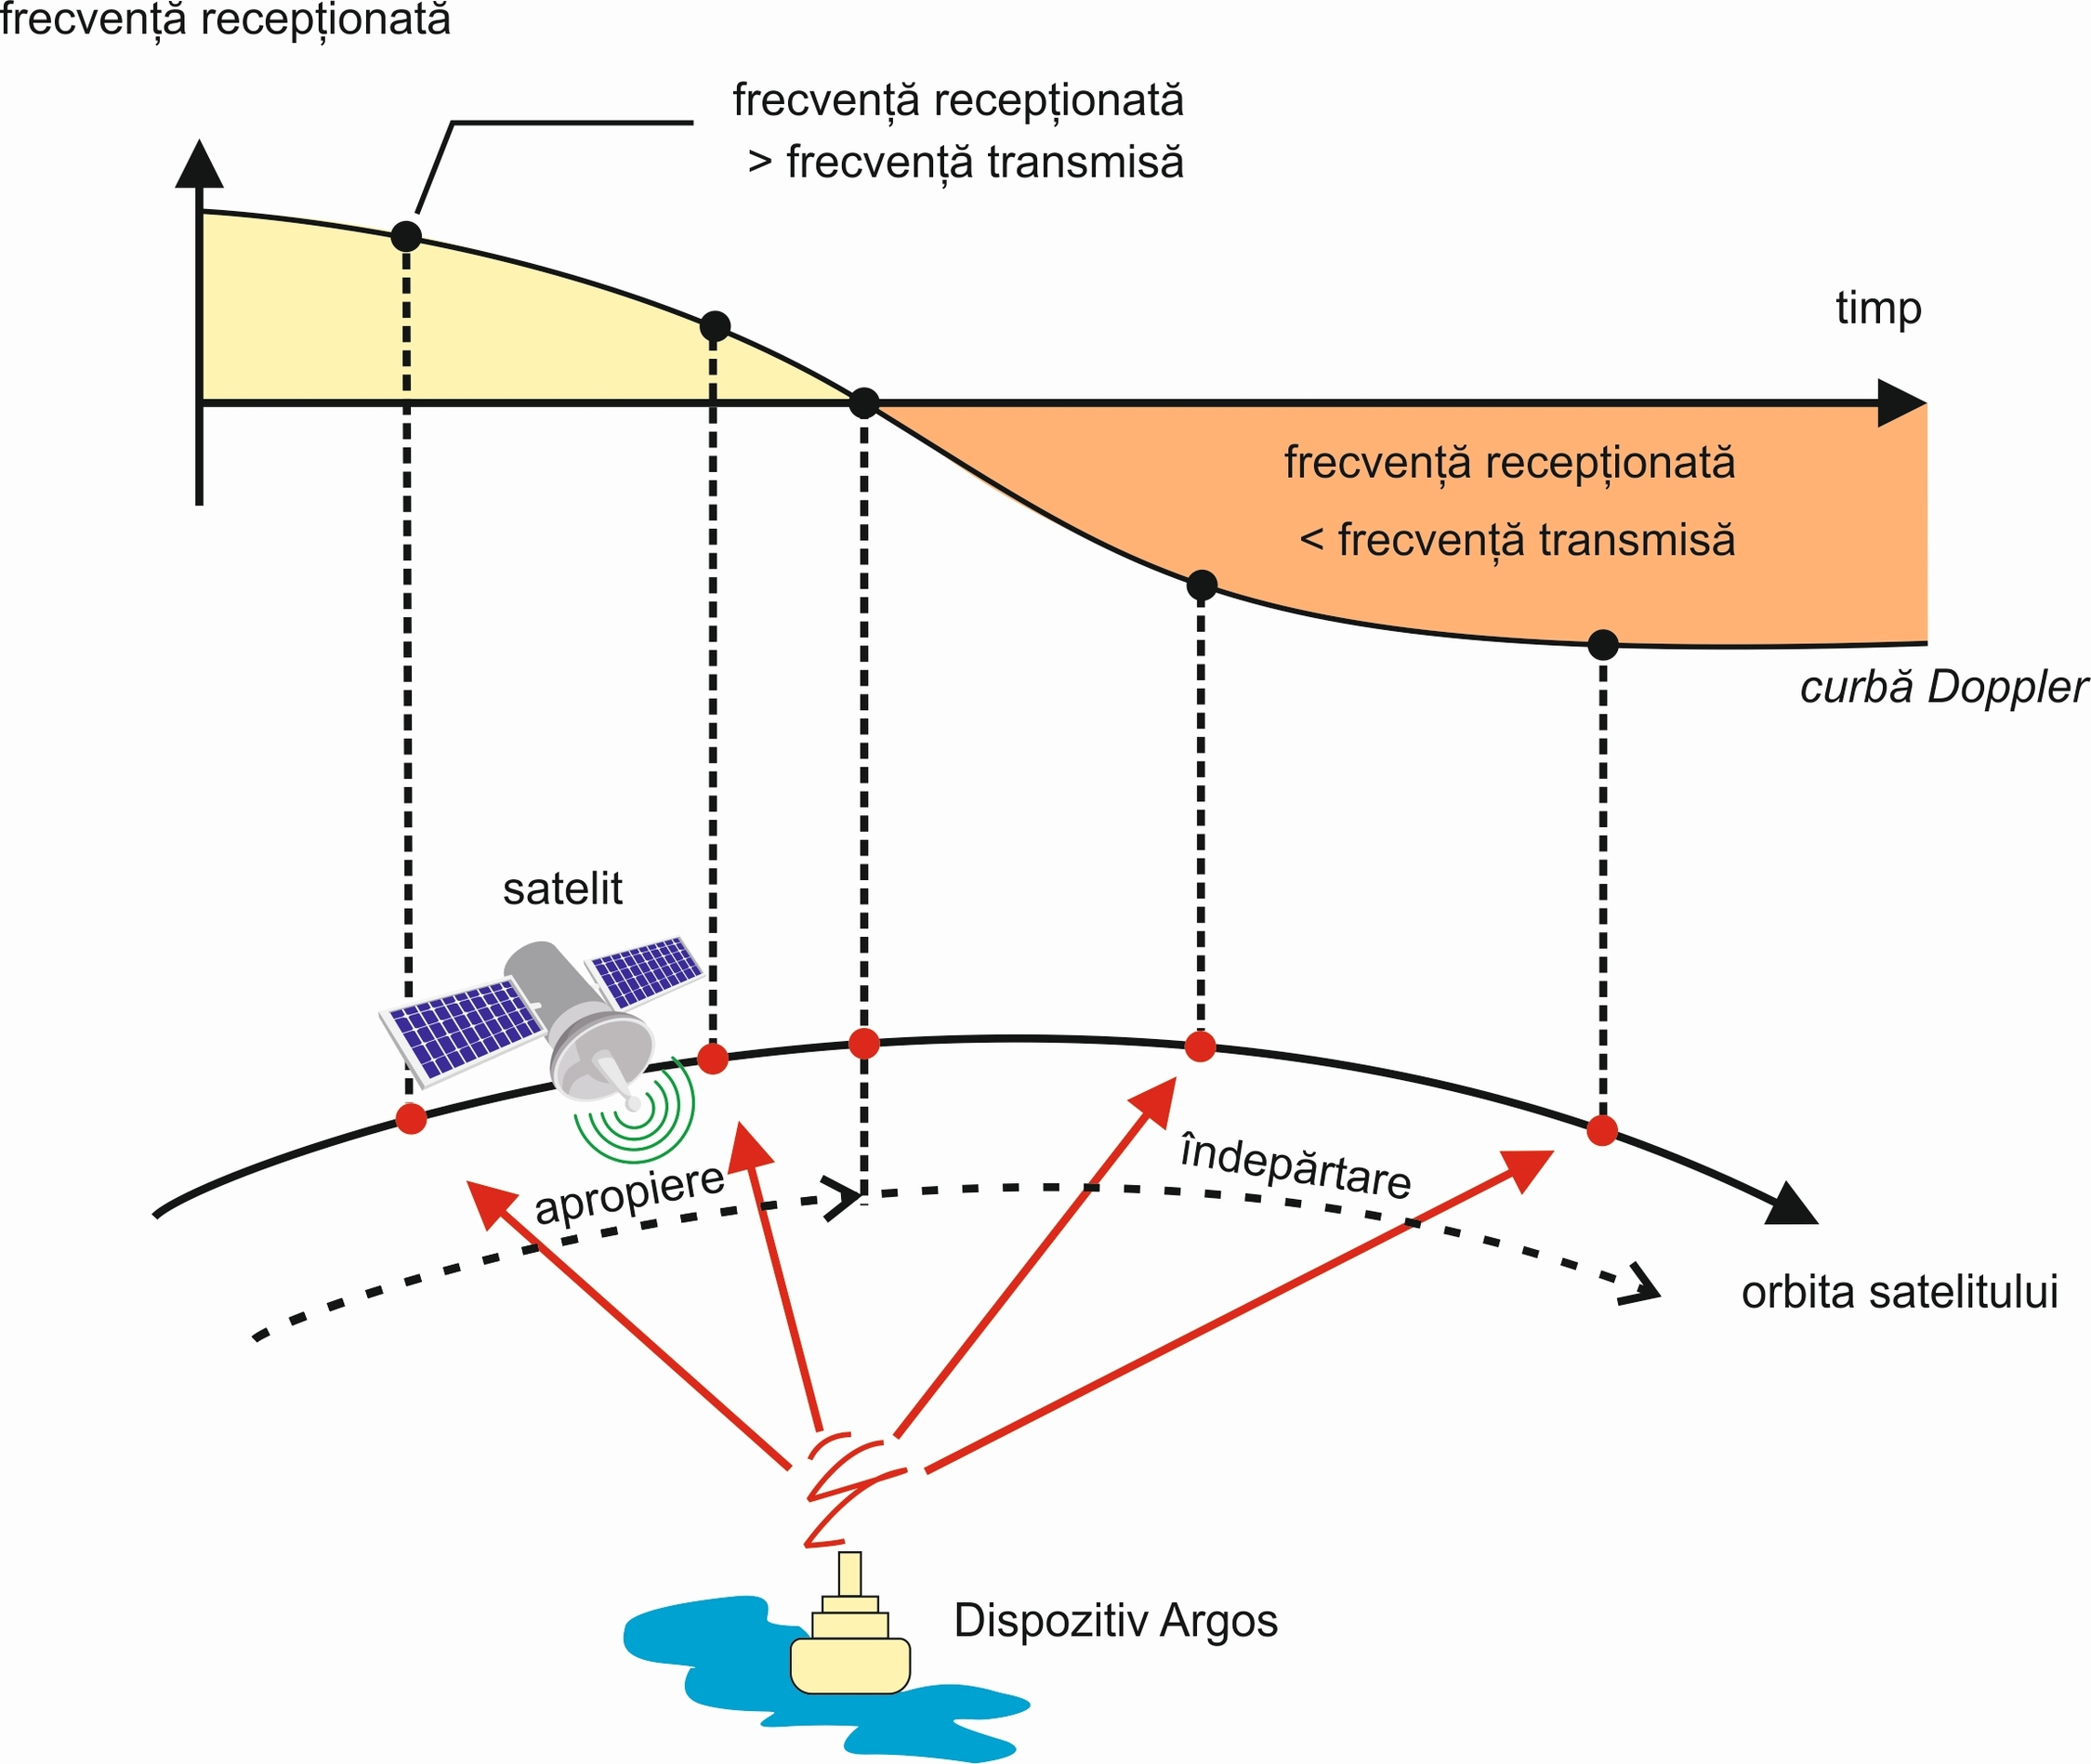
\includegraphics[width=\textwidth]{Fig2.jpg}
\caption{Funcționarea dispozitivelor pentru localizare Argos Doppler. Localizarea se face de unul din cei 6 sateliți cu instrumente Argos (© seaturtle.org).} \label{fig2}
\end{figure}
Poziția platformei este calculată prin unul din cei doi algoritmi CLS (Least-squares sau filtru Kalman, recomandat fiind Kalman datorită acurateței mai mari), funcție de viteza maximă/h estimată a platformei, adică a individului monitorizat (informație ce trebuie introdusă de utilizator la activarea platformei) \citep{Lopez2015,Lowther2015}. Localizarea este returnată utilizatorului prin platforma CLS cu informații precum: clasa de localizare, coordonatele geografice primare, soluția 2 de coordonate geografice (circa 3\% dintre coordonate se potrivesc mai bine soluției 2), diferiți parametri de estimare a erorii, altitudinea pe DEM USGS GTOPO30, valori ale senzorilor \citep{Douglas2012}. În cazul în care nu se poate stabili o localizare, atunci coordonatele geografice nu sunt transmise odată cu mesajul, fiind marcată ca localizare invalidă. Cea mai la îndemână măsură a acurateței este clasa de localizare: \textbf{LC3} (eroare estimată < 250m), \textbf{LC2} (eroare estimată 250m << 500m), \textbf{LC1} (eroare estimată 500m << 1500m), \textbf{LC0} (eroare estimată > 1500m, livrată la cerere), \textbf{LCA} (fără eroare estimată), \textbf{LCB} (fără eroare estimată), \textbf{LCZ} (localizare invalidă, livrată la cerere prin interpolare) și \textbf{LCG} (mesaje cu localizare GPS, dacă PTT-ul are și GPS încorporat) \citep{CLS2016}. Localizările LC3-LC0 sunt derivate din 4 sau mai multe mesaje, localizările LCA din 3 mesaje, iar localizările LCB din 1-2 mesaje \citep{CLS2016} (Figura ~\ref{fig3}).
\begin{figure}[ht]
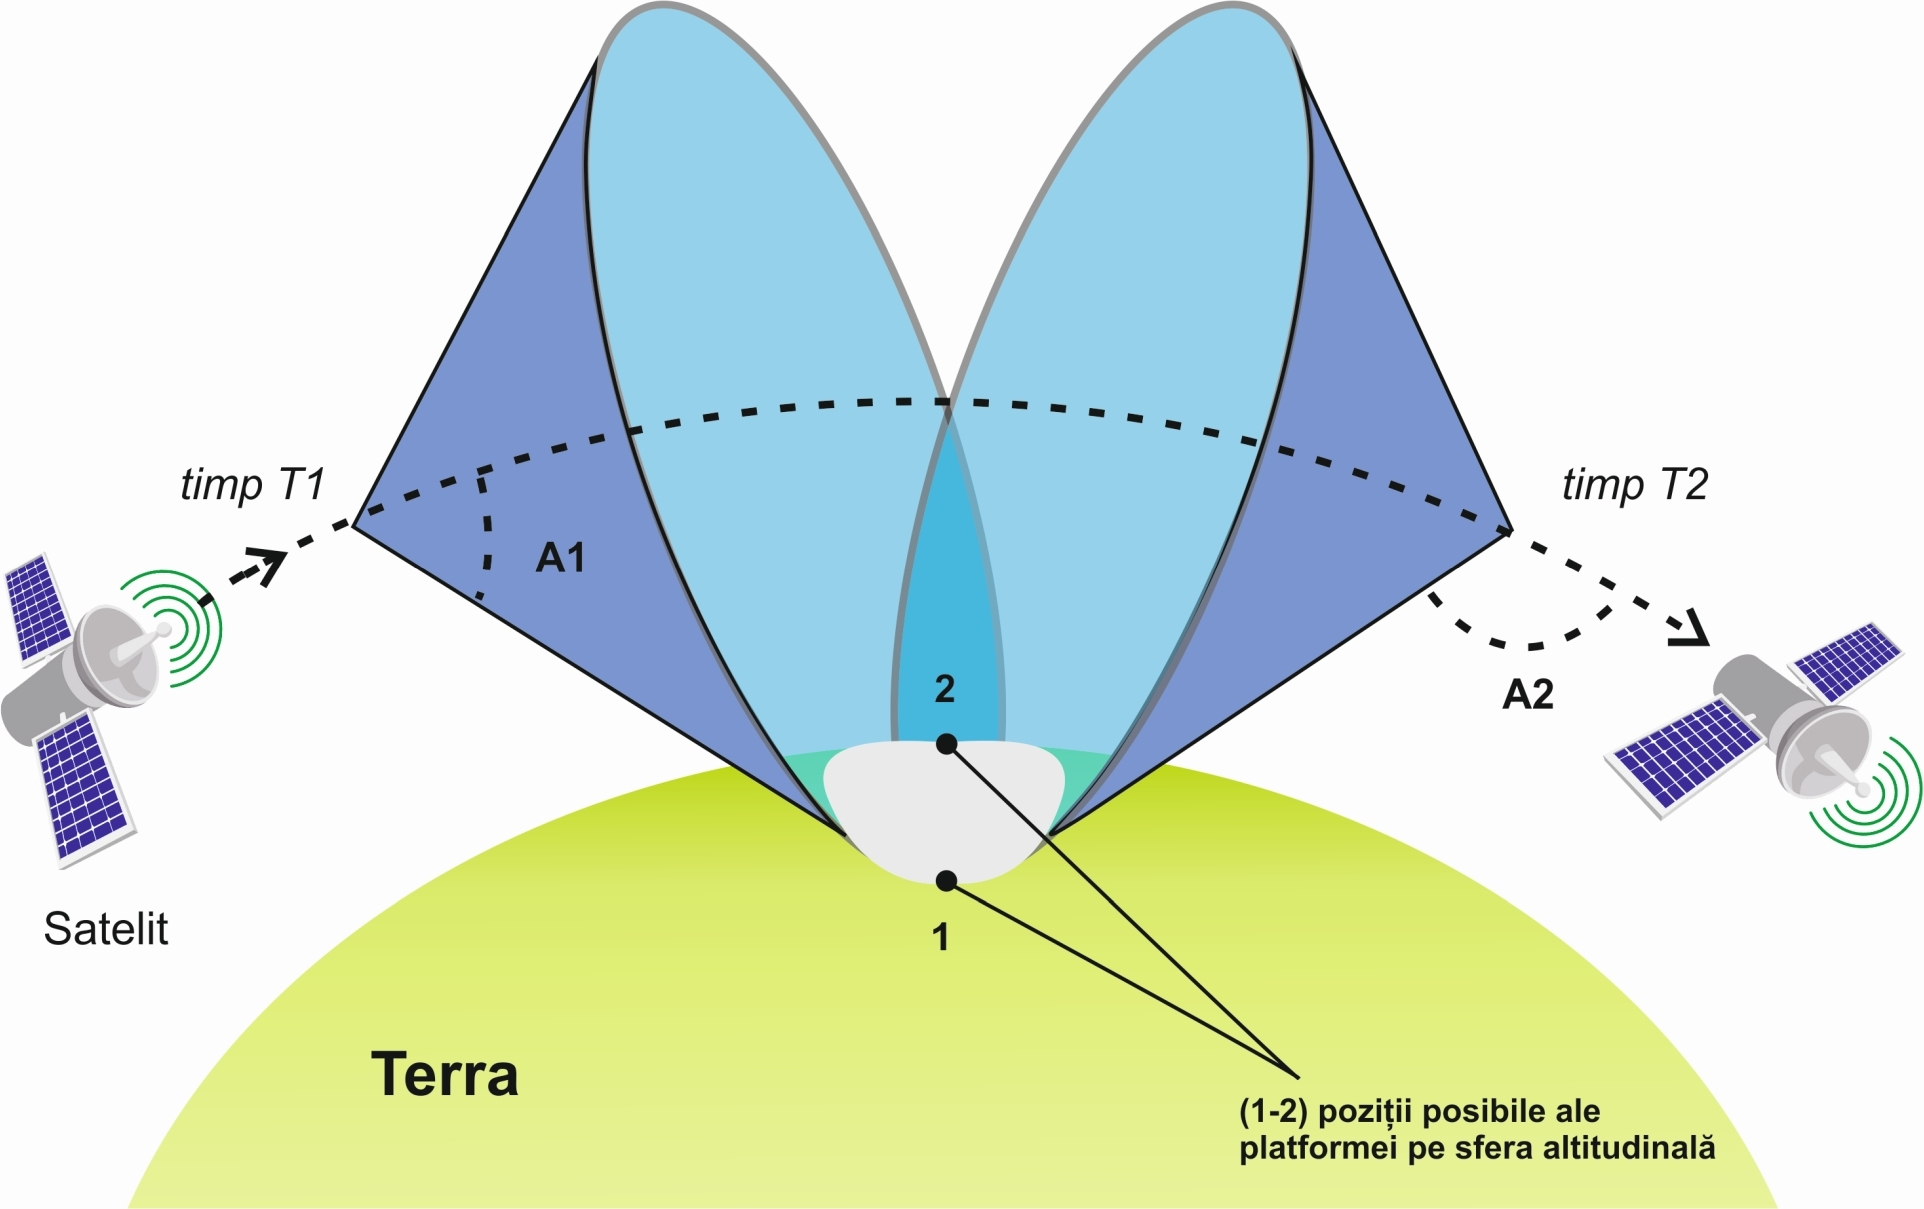
\includegraphics[width=\textwidth]{Fig3.jpg}
\caption{Localizarea Argos Doppler. Sistemul analizează schimbarea frecvenței semnalului transmis de PTT prin mișcarea concomitentă a dispozitivului și satelitului și produce două soluții de localizare (© CLS Argos).} \label{fig3}
\end{figure}

Platforma Argos poate avea înglobat un GPS (PTT-GPS), astfel că unele mesaje (clasa G) sunt de precizie GPS, sub 10m. Platformele cu GPS sunt mai grele, cele mai mici au peste 25g, comparativ cu sub 5g în cazul PTT-ului simplu. CLS va procesa mesajele Argos folosind coordonatele GPS dacă din punct de vedere temporal sunt compatibile, crescând precizia localizărilor Doppler \citep{CLS2016}.

Platformele Argos sunt echipate cu microcontrolere ON/OFF (pentru activarea după un număr de ore în care semnalul radio se oprește), pot avea panou solar pentru alimentare cu energie, transmițător VHF/UHF pentru senzorul de mortalitate și localizarea în teren după desprinderea de animal, alți senzori cum ar fi accelerometru, temperatură, lumină, presiune, GPS etc. Pentru speciile marine, GPS-ul este unul de tip FastLock care pot produce localizări GPS într-o perioadă foarte scurtă de timp, când individul iese la suprafața \citep{Lowther2015}. Sunt disponibile cu prindere tip rucsac (Figura ~\ref{fig4}), lipite, atașate de membre, pene, colier.
\begin{figure}[ht]
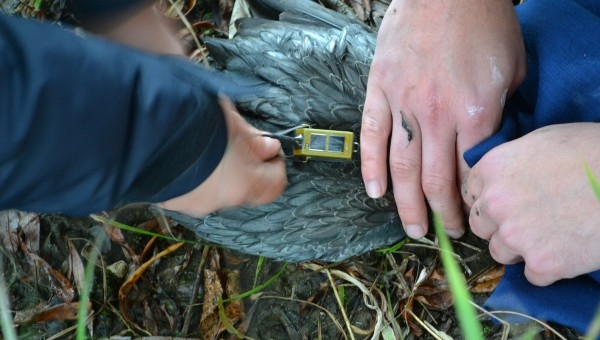
\includegraphics[width=\textwidth]{Fig4.jpg}
\caption{Dispozitiv PTT Argos 9.5g tip rucsac montat pe cormoran mic (proiect LIFE10 NAT/RO/00740).} \label{fig4}
\end{figure}

Costurile echipamentelor sunt ridicate dar nu necesită prezență permanentă în teren. Numărul de localizări precise este mai mic comparativ cu cel furnizat de echipamentele cu sisteme GPS, dar tehnologia este foarte utilă pentru studiul speciilor migratoare sau marine.

\subsection{Geolocație prin măsurarea nivelului de lumină}

Geolocalizarea prin măsurarea nivelului de lumină este o tehnică de monitorizare relativ recentă. Folosită inițial pentru specii marine, a căpătat popularitate pentru monitorizarea speciilor de păsări migratoare de dimensiuni mici \citep{Silvy2012}. Geolocatoarele au un senzor electronic de lumină prin care înregistrează nivelul de lumină într-un moment predefinit, iar uneori senzori de temperatură, presiune, accelerometru etc. Datele sunt arhivate on board sau pot fi transmite prin uplink sau radio dacă dispozitivele sunt mai mari și au surse de energie mai puternice. Dispozitivele sunt de dimensiuni mici, pot avea sub 2 grame și se pot monta lipite sau tip rucsac \citep{Bridge2011} (Figura ~\ref{fig5}). Dispozitivele care au și senzori de presiune pot fi implantate (de exemplu, pentru pești).
\begin{figure}[ht]
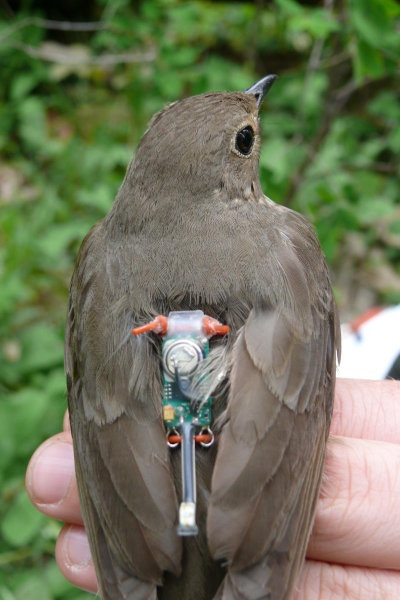
\includegraphics[width=9cm]{Fig5.jpg}
\caption{Geolocator tip rucsac (© Kira Delmore, UBC).} \label{fig5}
\end{figure}

Metoda principală de localizare este “threshold”, care înregistrează momentele de răsărit și apus, după care raportează datele la valorile specifice fiecărei zone de pe glob. O altă metodă este ”template fit” care măsoară forma tranziției luminii între răsărit și apus. Astfel, aceasta necesită o perioadă completă de observații, nu numai în două momente ale zilei ca la metoda "threshold" (Bridge 2013). Erorile spațiale produse de geolocatoare sunt mult mai mari decât la celelalte sisteme, în medie de circa 150 km, iar prelucrarea și calibrarea datelor necesită cunoștințe speciale \citep{Silvy2012} (Figura ~\ref{fig6}).
\begin{figure}[ht]
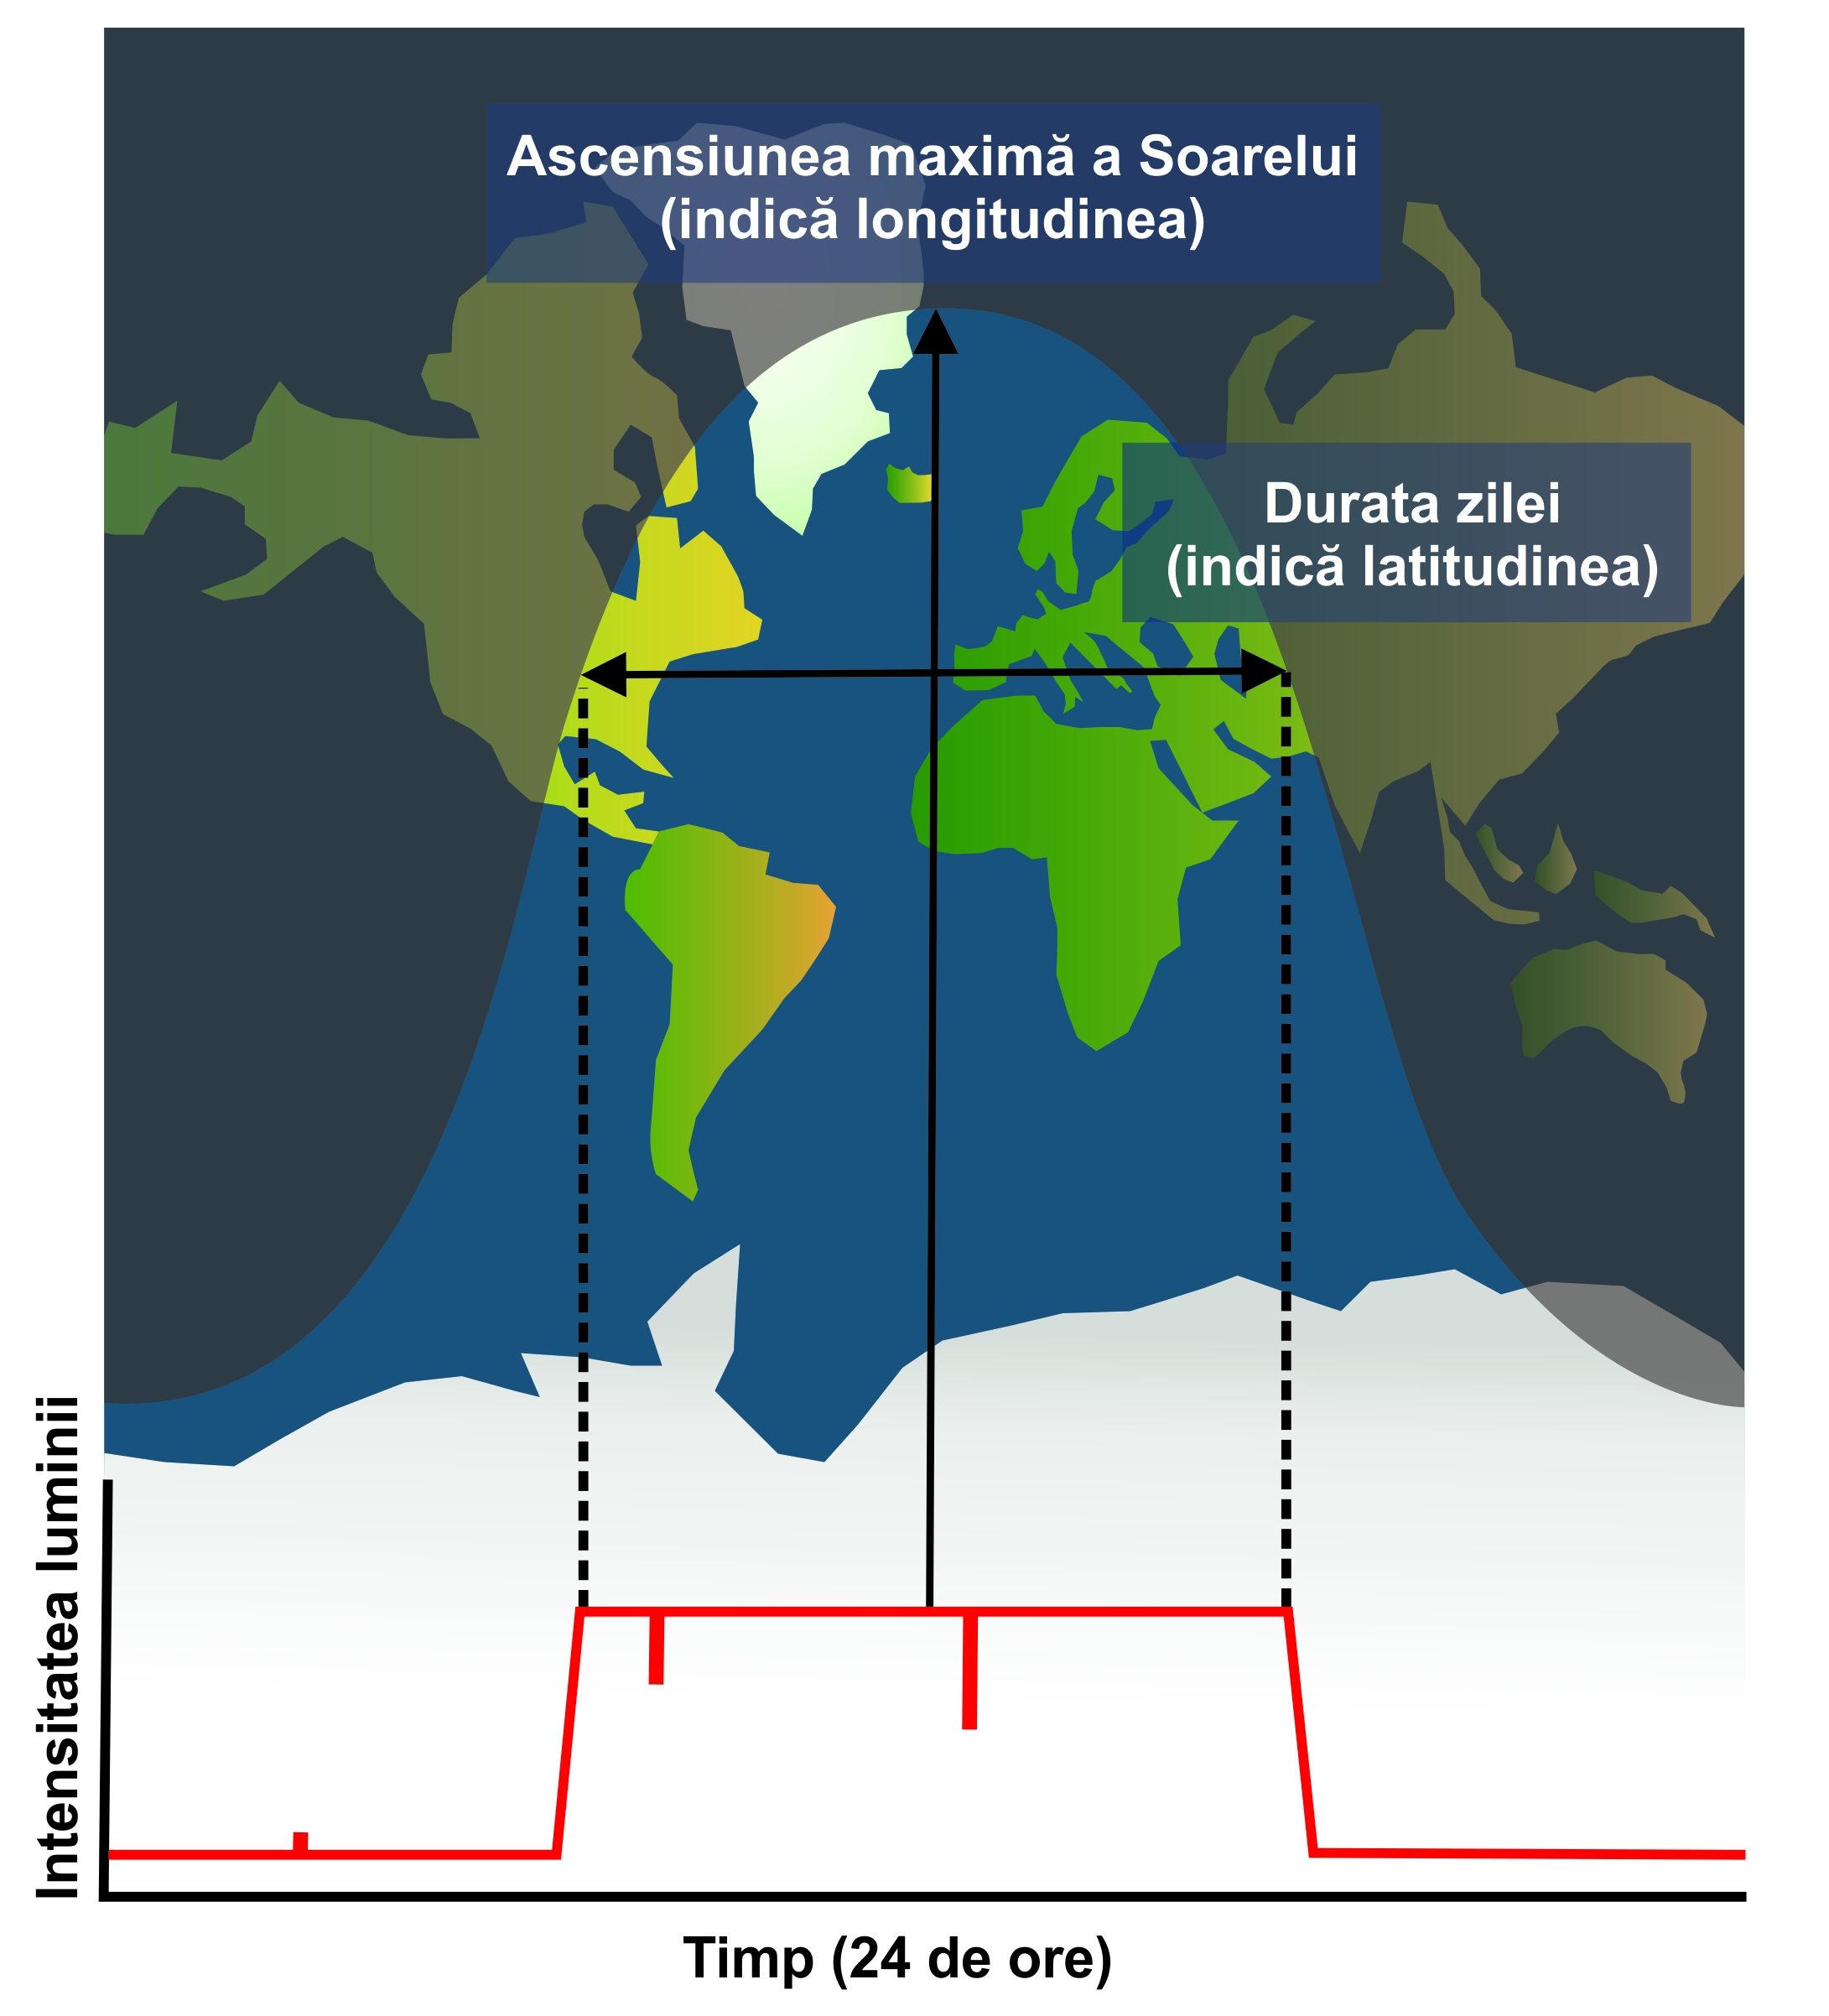
\includegraphics[width=12cm]{Fig6.jpg}
\caption{Principiul localizării prin geolocatoare de lumină (© University of Oklahoma, Animal Migration Research Group)} \label{fig6}
\end{figure}

Costurile echipamentelor sunt mici, dar necesită recuperarea acestora dacă nu sunt prevăzute cu sisteme de transmisie date. Este o metodă utilă pentru studiul migrațiilor la specii de dimensiuni mici.

\section{Selectarea tehnologiei optime pentru localizare} 

Deși fiecare cercetător și-ar dori să producă un volum mare de date precise utilizând tehnologie actuală, acest lucru nu este întotdeauna posibil din cauza unor constrângeri tehnologice, ecologice sau financiare. Principalele elemente de care trebuie să ținem cont la selectarea tehnologiei de monitorizare sunt \citep{Silvy2012, Thomas2012}:
\begin{itemize}
 \item \textbf{Greutatea indivizilor de monitorizat.} Echipamentele precise de tip GNSS (GPS), mai ales cele cu sisteme de descărcare de date de la distanță, necesită o sursă mare și constantă de energie, crescând astfel greutatea acestora. Cum echipamentele de localizare nu ar trebui să depășească 5\% din greutatea individului monitorizat, opțiunile de localizare precisă pentru speciile mici sunt limitate.\\
 \item \textbf{Comportamentul.} Unele specii petrec mult timp în spații închise (peșteri), fără soare (latitudini mari, pădure), în apa mării etc. Aceste comportamente aduc restricții de localizare, de exemplu, dacă există recepție Argos sau GPS, expunere la soare suficientă pentru bateria cu reîncărcare solară, posibilitatea recapturării, specii statice, distanțele parcurse etc. De exemplu, receptoarele Argos nu se pretează la specii care se deplasează pe distanțe mici (e.g., țestoase terestre).\\
\item \textbf{Numărul de poziții și calitatea acestora.} Dacă studiul necesită obținerea unui număr mare de poziții sau o calitate bună a acestora, atunci se vor alege echipamentele adecvate acestor deziderate (e.g., GPS pentru multe poziții precise, Argos pentru multe poziții mai puțin precise). În unele cazuri se va constata că nu există nici un echipament care să poată asigura astfel de cerințe (de exemplu, cele existente sunt prea grele), caz în care se vor studia metodele de postprocesare a datelor și se vor adapta obiectivele de cercetare în consecință.\\
 \item \textbf{Modalitatea de prindere a dispozitivelor de localizare.} Configurația dispozitivelor depinde și de conformația speciei de interes. Astfel, receptorul GPS trebuie să fie plasat o perioadă cât mai îndelungată spre cer, panoul solar să nu fie obturat de pene sau blană, panoul solar să nu poată fi deteriorat de animal, să nu existe o creștere mare a individului (de exemplu a circumferinței gâtului, volumului corpului).\\
\item \textbf{Caracteristicile morfologice ale terenului și echiparea tehnică a arealului de studiu.} În unele zone, recepția GPS sau Argos este foarte slabă (văi adânci), astfel că dacă indivizii stau o perioadă lungă în astfel de condiții, localizările vor fi cu precizie scăzută iar durata de viață a dispozitivelor va fi mai mică din cauza consumului mare de energie necesar încercărilor succesive de localizare. Mai mult, dacă individul nu se deplasează către zone cu recepție, datele stocate on board pot fi pierdute.\\
 \item \textbf{Costurile și resursele umane necesare.} Studiile de localizare includ cinci categorii de costuri: costurile pentru capturarea indivizilor ce urmează a fi monitorizați, costurile echipamentelor, costurile de transmisie-recepție date, costurile de prelucrare a datelor, costurile cu permisele de lucru. Fiecare dintre aceste categorii de costuri necesită flux constant de bani. Costurile echipamentelor și transmisiei trebuie verificate întotdeauna cu producătorii, iar estimarea trebuie să acopere o perioadă suficient de mare de timp pentru a îndeplini obiectivele. Estimarea trebuie să includă toate taxele (asigurări, TVA, taxe vamale, transport). În plus, în fiecare perioadă trebuie să avem resurse umane care să poată îndeplini obiectivele (e.g., personal cu expertiză în capturat animale care să poată o călători perioadă îndelungată), echipamente (cuști, plase, tranchilizante, mașină etc). Capturarea animalelor este poate cea mai dificilă etapă și în general pentru un număr mare de animale este necesară o perioadă lungă de timp. Uneori este necesară o perioadă de peste 1 an pentru capturare, altfel că dispozitivele de localizare deja achiziționate nu mai au suficientă energie pentru a fi utilizate o perioadă mai mare de timp (de exemplu, un GPS drop-off montat la 1 an de la achiziție se poate descărca după 3-4 luni de funcționare). Astfel, decizia finală trebuie luată și în funcție de existența acestor resurse.
\end{itemize}

După greutate și sursa de energie, dispozitivele de localizare pot fi (Tabel ~\ref{tab:1}, Figura ~\ref{fig7}) \citep{Thomas2012}:
\begin{table}[h!]
\caption{\label{tab:1}Caracteristici ale dispozitivelor de localizare.}
\begin{tabular}{ m{3cm}  m{2cm}  m{1.8cm}  m{4cm}  m{3cm} }
\midrule
\textbf{Tip echipament} & \textbf{Greutate min. (g)} & \textbf{Sursa energie} &	\textbf{Număr poziții} &	\textbf{Greutate min. specie (g)}\\
\midrule
VHF & 0.2 &	Baterie	& 1 an & 9\\
Geolocatoare & 0.5 & Baterie	& Depinde de frecvența localizării & 18\\
GPS store on board & 1 & Baterie	& 50 & 35\\
Argos Doppler & 5 & Solar & Nelimitat & 170\\
GPS radio & 5 & Baterie & 500 & 170\\
Argos Doppler GPS & 17 & Solar & Nelimitat & 570\\
GPS GSM & 25 & Solar & Nelimitat & 840\\
GPS Iridium/ Globalstar & 130 & Baterie & Depinde de frecvența localizării & 4400\\
\midrule
\end{tabular}
\end{table}
\begin{figure}[ht]
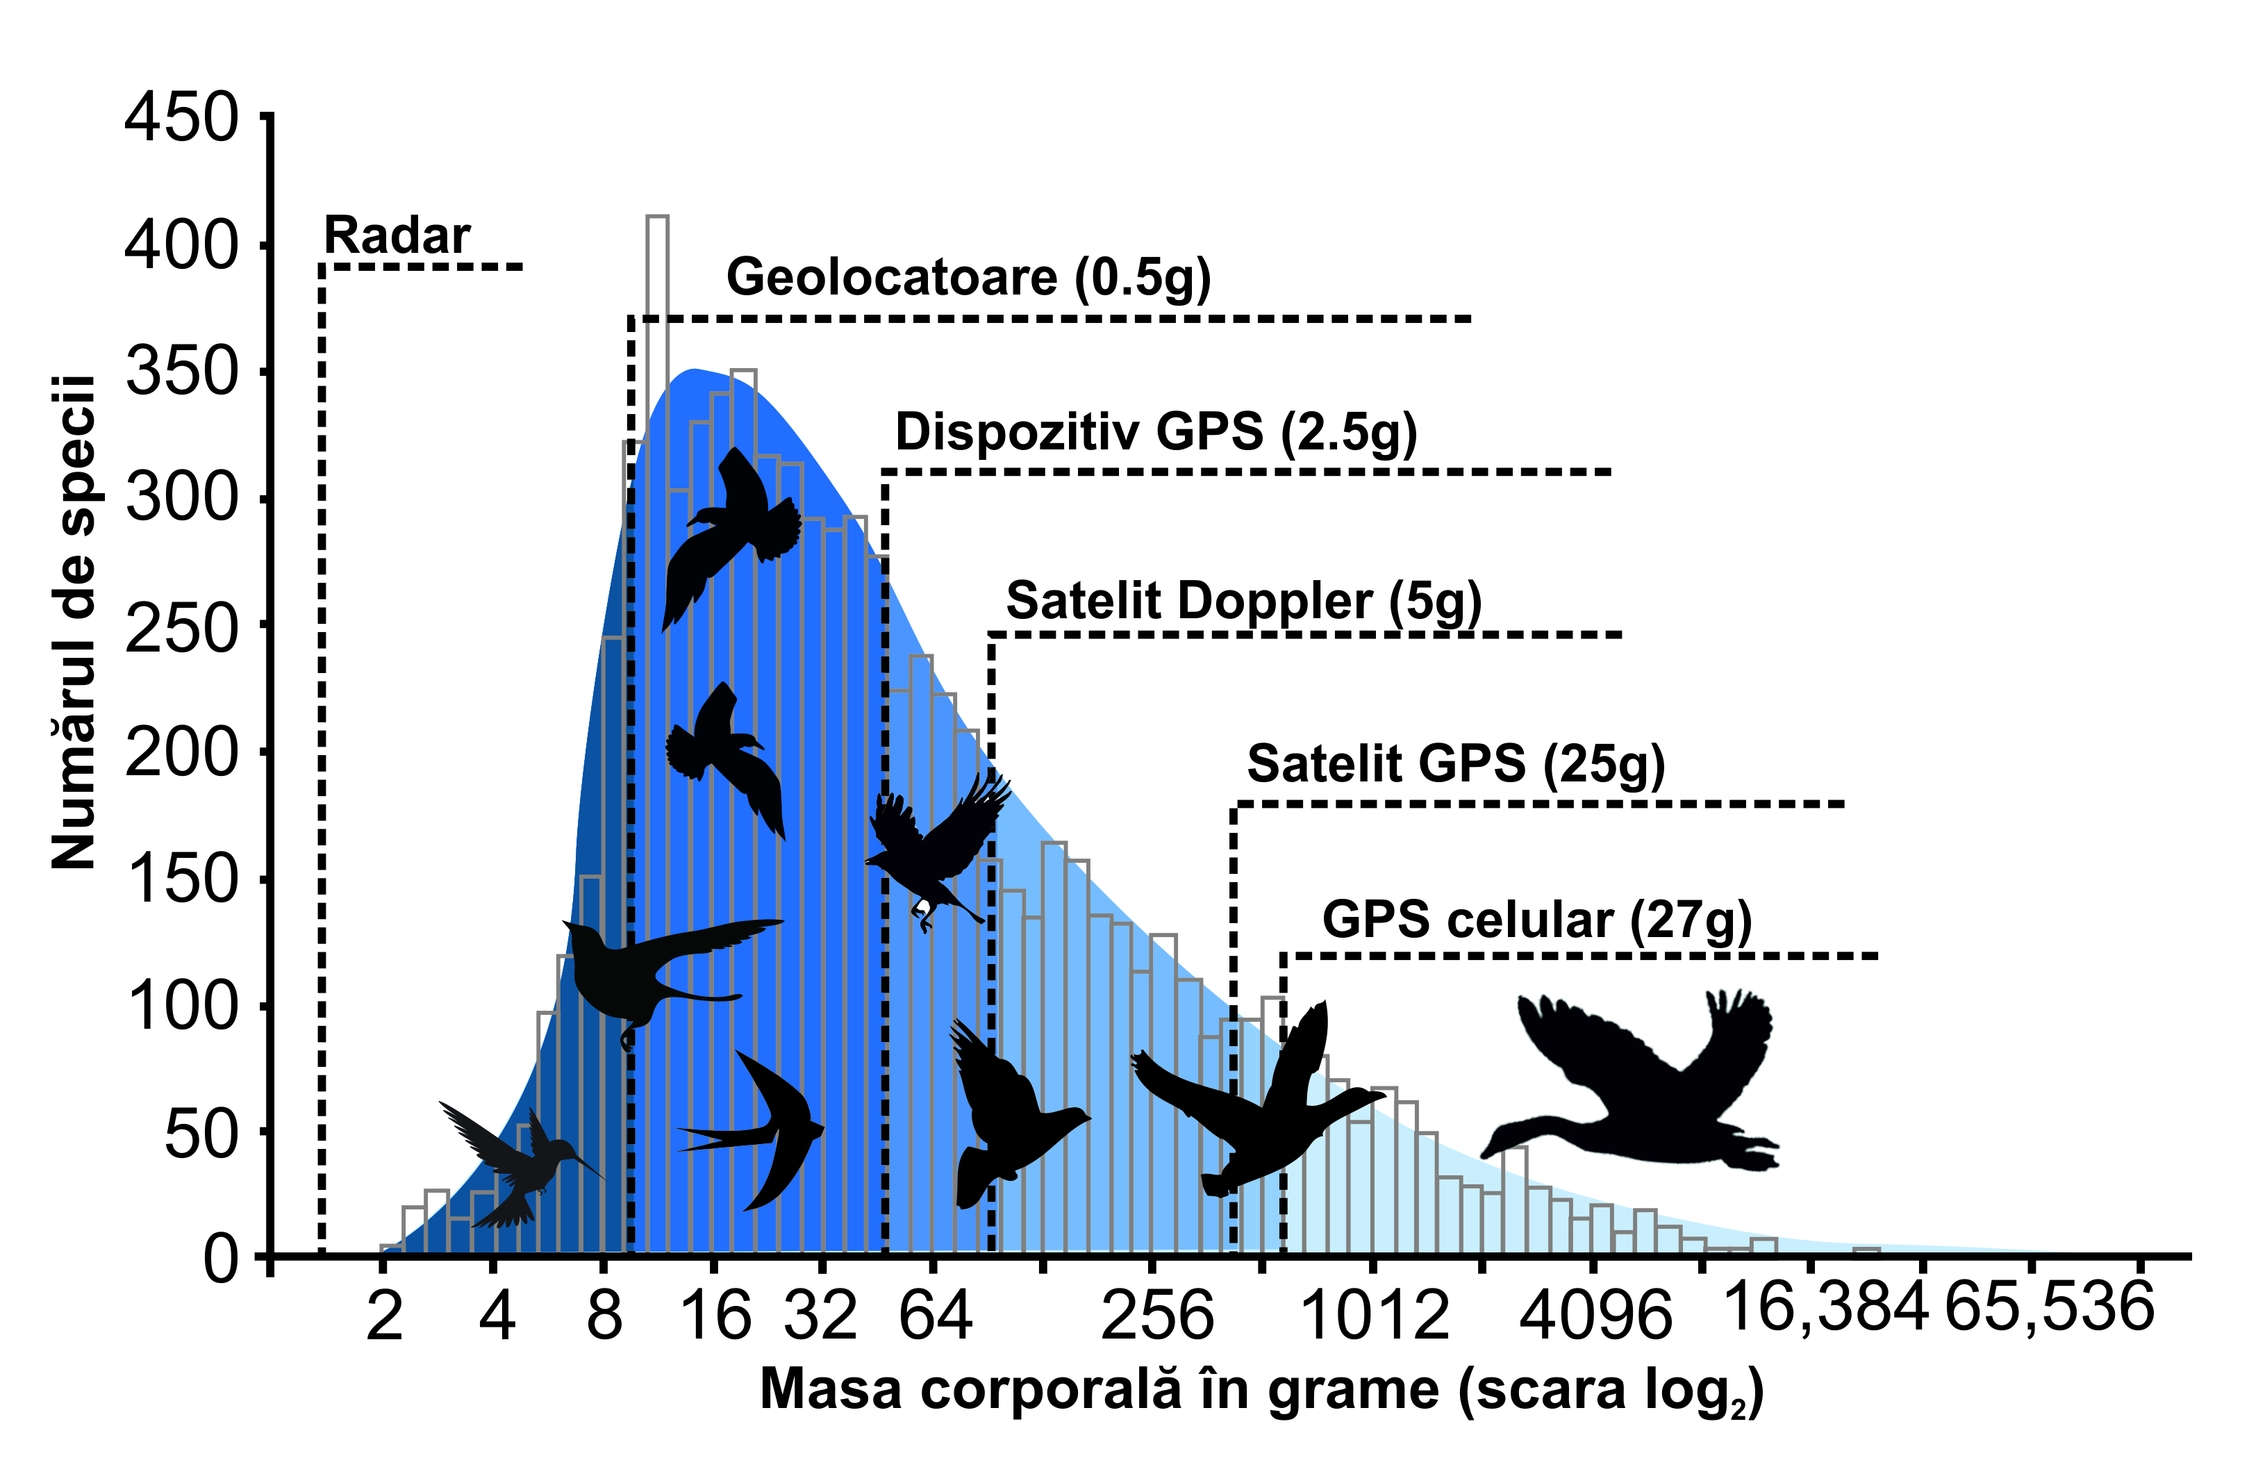
\includegraphics[width=\textwidth]{Fig7.jpg}
\caption{Numărul de specii de păsări ce pot fi monitorizate cu diferite tehnologii de localizare. Limita maximă a fost considerată la 5\% din greutatea corpului \citep{Bridge2011}} \label{fig7}
\end{figure}

După tipul de atașare pe animal, dispozitivele de localizare pot fi \citep{Silvy2012}:
\begin{itemize}
    \item \textbf{Lipit.} Lipit cu epoxy, pe carapace, pe piele, pe penele unor pasări, în zona scapulară.
  \item \textbf{Tip rucsac pe spate.} Trebuie create bretele din bandă de teflon (se adaugă cel puțin 2 grame, Figura ~\ref{fig8}).
    \item \textbf{Subcutanat.} Se atașează prin implant chirurgical, antena trebuie purtată în afară.
    \item \textbf{Colier de gât sau picior.} Se atașează de gâtul sau piciorul animalului cu un colier de plastic sau lipit de picior cu epoxy.
    \item \textbf{Cârlig în piele (prong and suture).} Pentru păsări, studii de scurtă durată, cum ar fi la cuibărit.
    \item \textbf{Pe coadă.} Pentru păsări.
    \item \textbf{Crotal pe aripă (patagial).} Utilizat pentru specii mari (Figura ~\ref{fig9}).
    \item \textbf{Pe picior cu teflon sau curea de piele (Tarsal-Jess).} Mai ales pentru specii de păsări răpitoare.
    \item \textbf{Crotal în ureche.} Pentru speciile de dimensiuni mari.
    \item \textbf{Guler (collar).} Util mai ales la speciile care au variații mari a circumferinței gâtului (Figurile ~\ref{fig10} și ~\ref{fig11}).
\end{itemize}
\begin{figure}[ht]
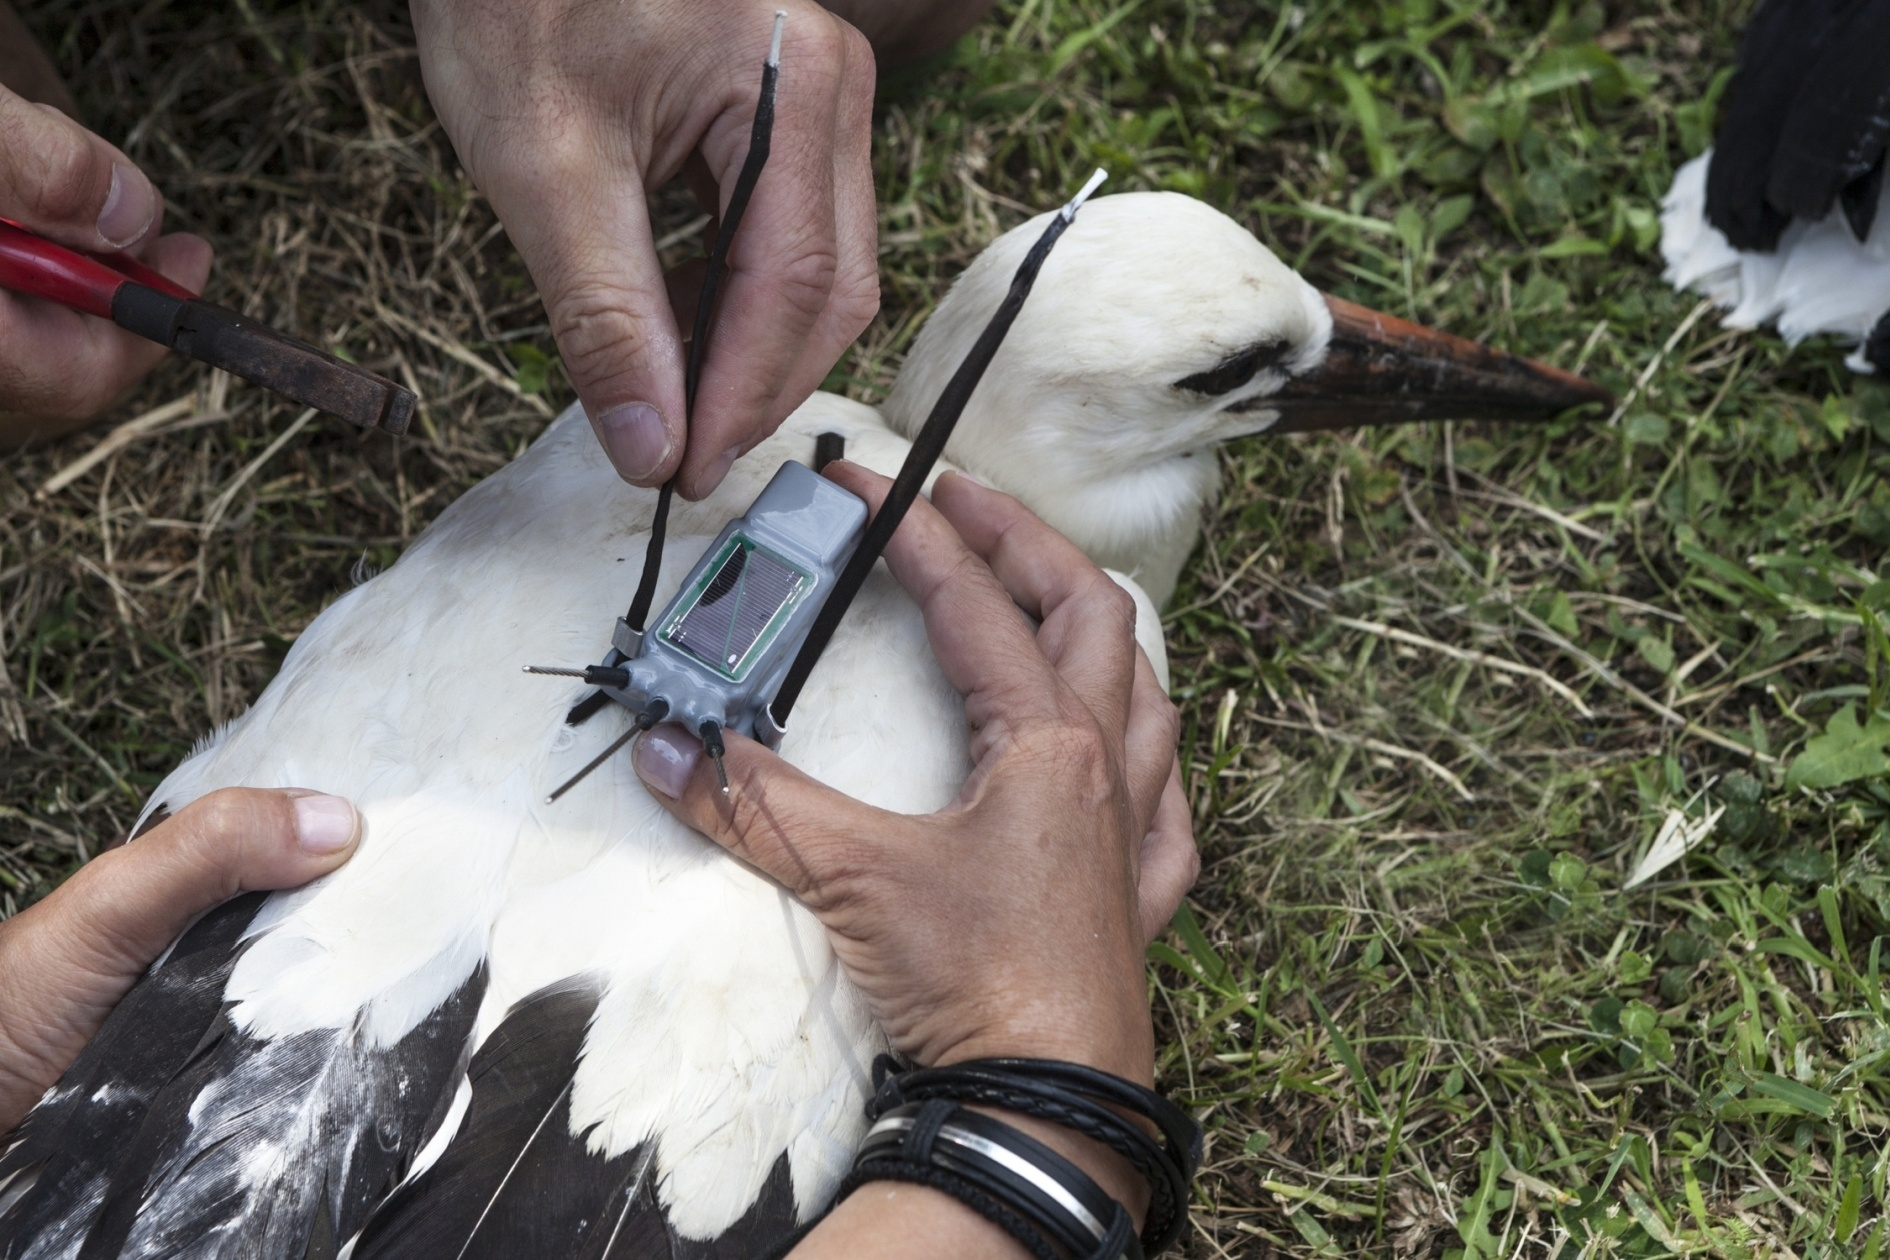
\includegraphics[width=\textwidth]{Fig8.jpg}
\caption{PTT solar cu GPS cu montaj tip rucsac (© Shutterstock).} \label{fig8}
\end{figure}
\begin{figure}[ht]
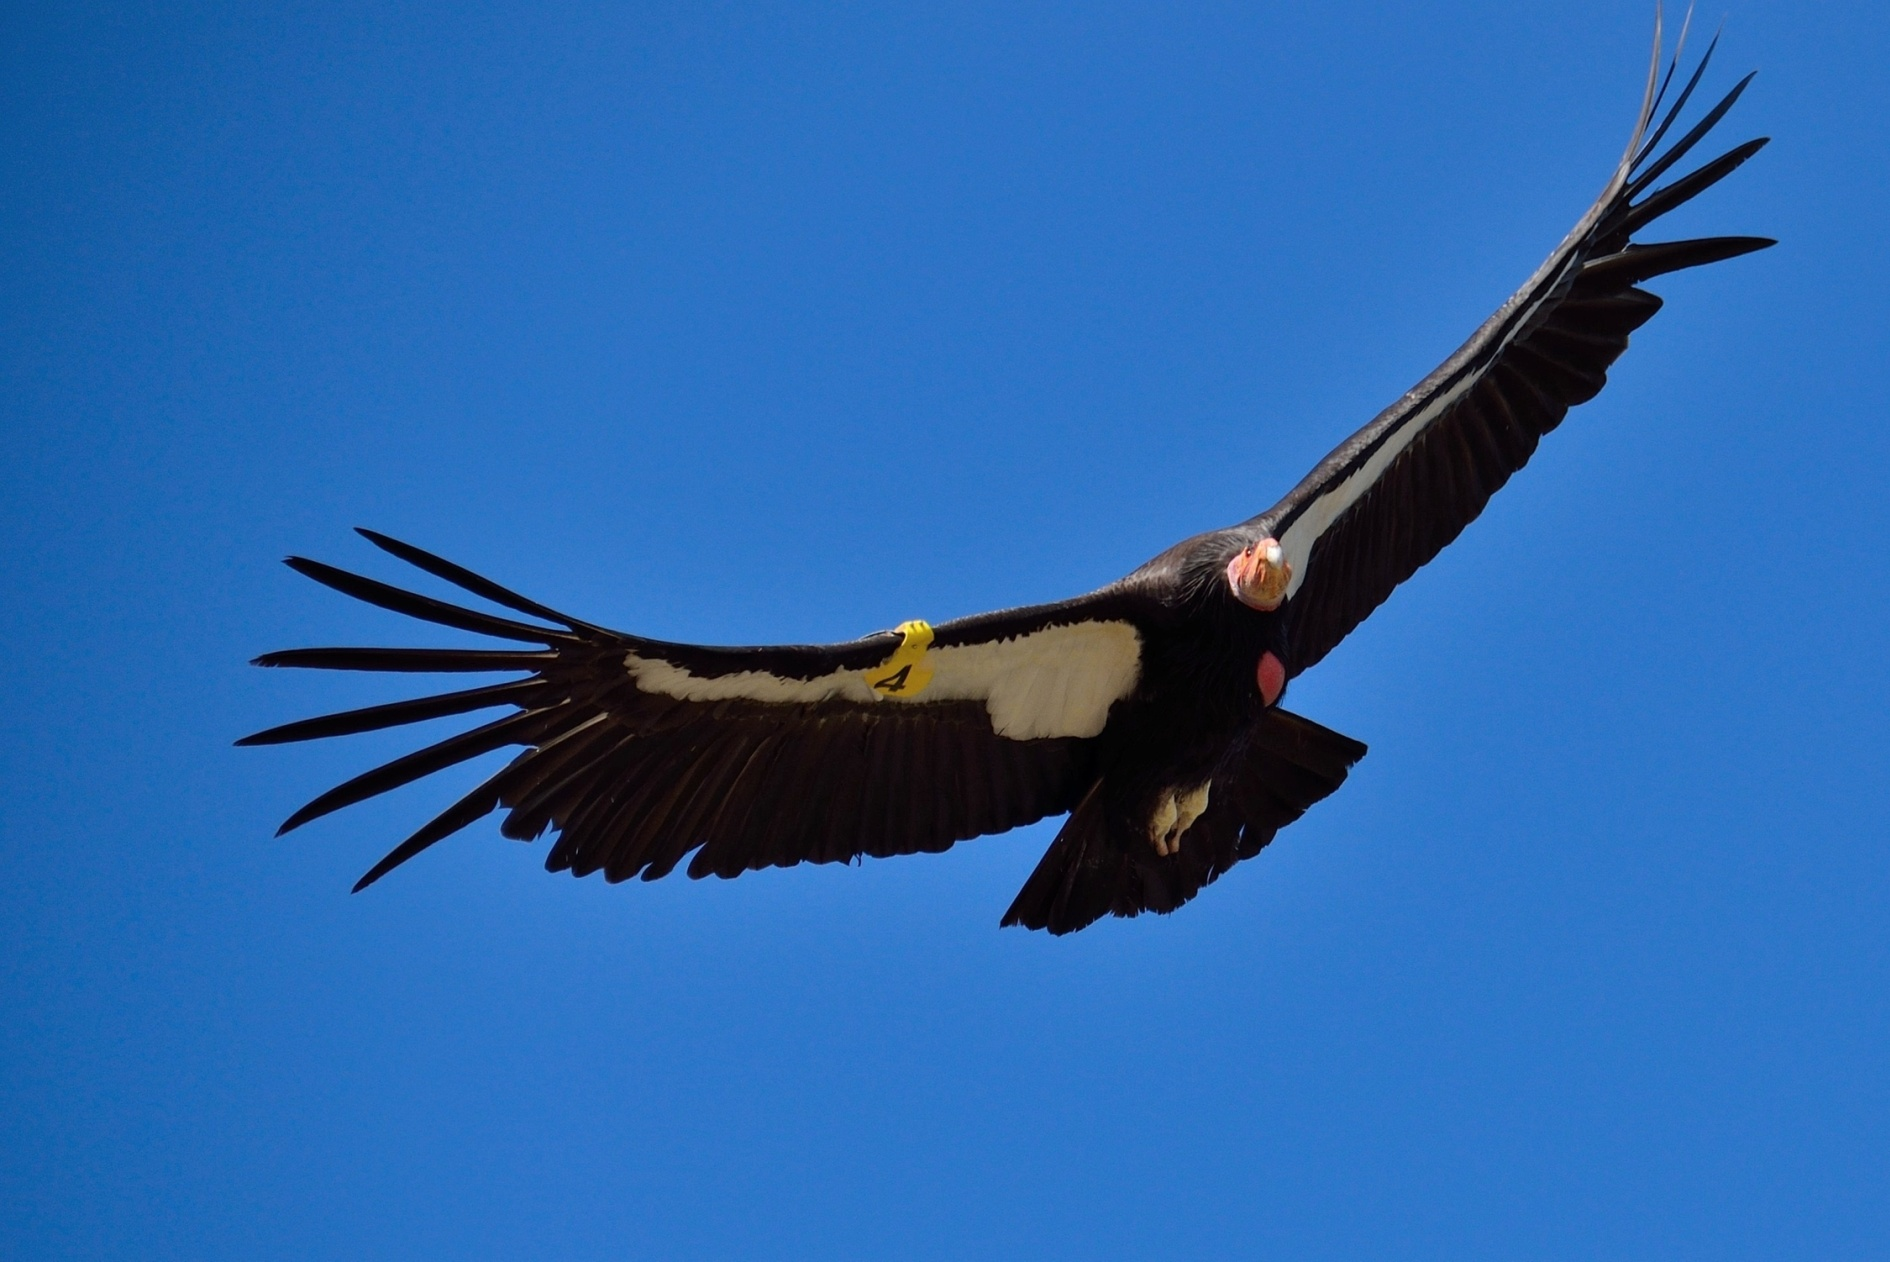
\includegraphics[width=\textwidth]{Fig9.jpg}
\caption{Dispozitiv de localizare montat patagial (© Shutterstock).} \label{fig9}
\end{figure}
\begin{figure}[ht]
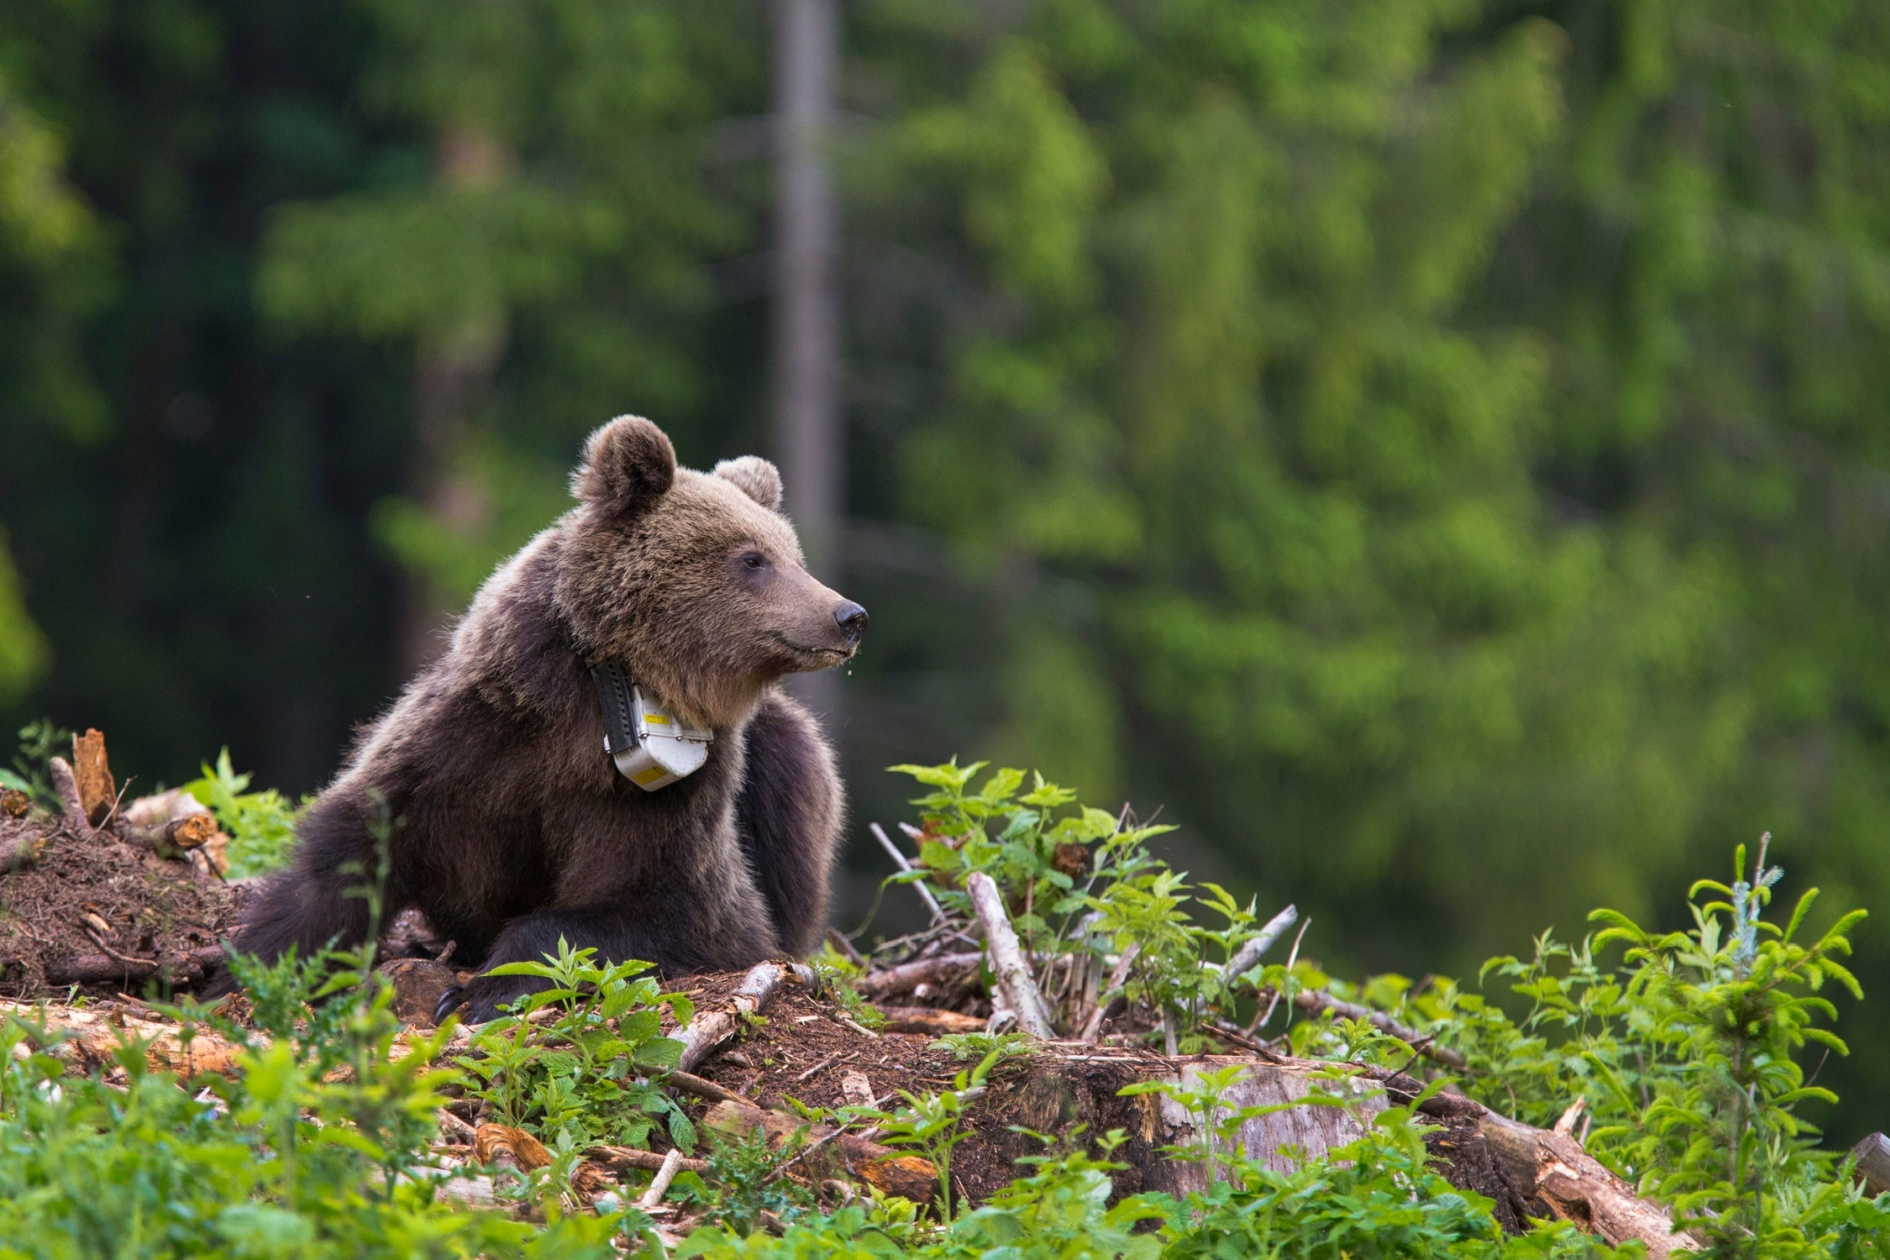
\includegraphics[width=\textwidth]{Fig10.jpg}
\caption{Dispozitiv de localizare tip colier montat pe urs brun (© Shutterstock).} \label{fig10}
\end{figure}
\begin{figure}[ht]
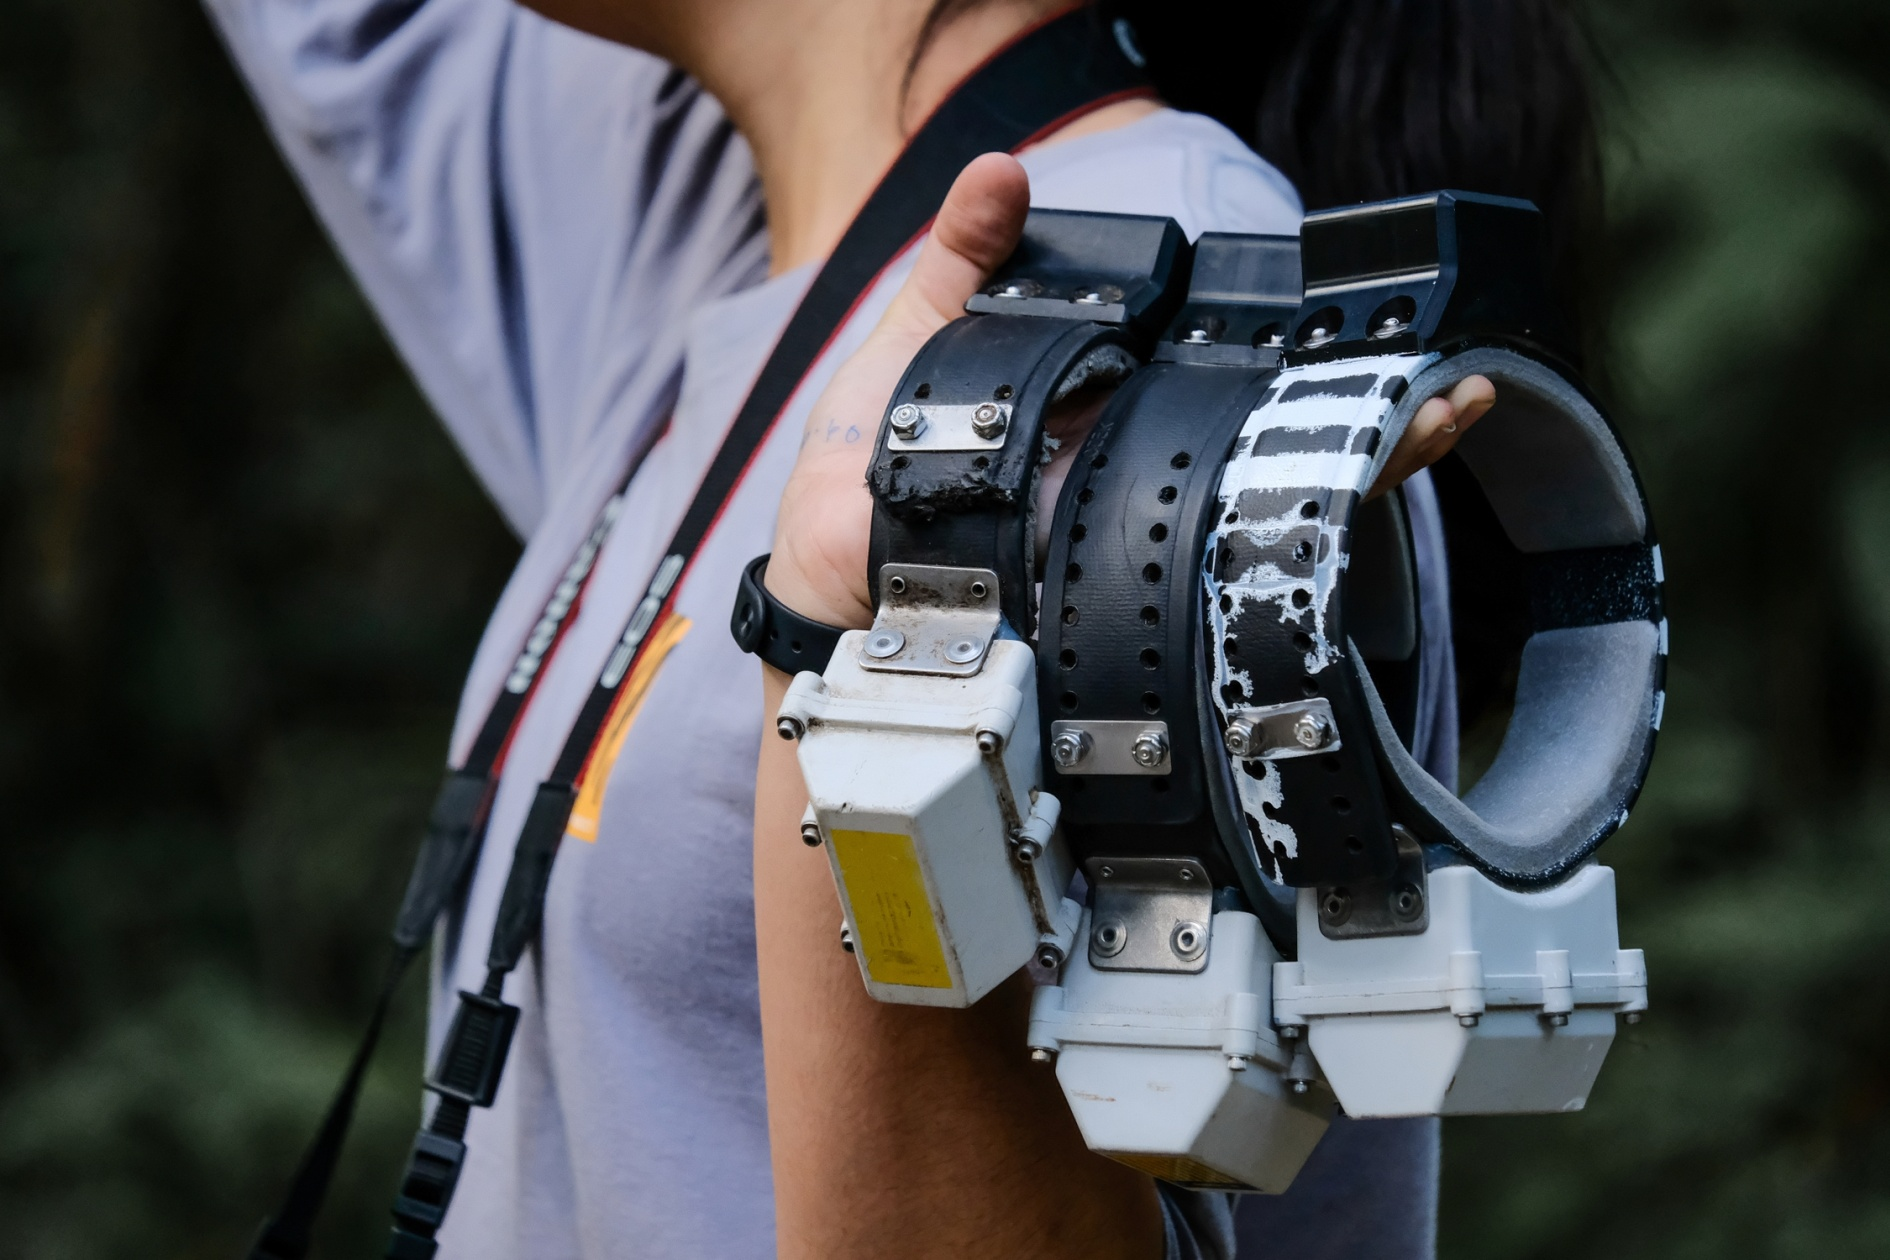
\includegraphics[width=\textwidth]{Fig11.jpg}
\caption{Dispozitive de localizare tip GPS colier cu sistem drop-off (© Shutterstock).} \label{fig11}
\end{figure}

Pentru dispozitivele cu panou solar, poziția panoului trebuie să fie mereu înspre cer, panoul nu trebuie să fie acoperit de pene sau blană sau accesibil ciocului păsării. De asemenea, panoul solar nu este potrivit la speciile care se deplasează în zona polară, hibernează sau intră în locuri fără lumină pe perioade mai mari de 4-5 zile (peșteri, vizuini etc.). Pentru o bună funcționare, ciclul ON va fi scurt (e.g., 8 ore) iar cel OFF lung (e.g., 43 ore). Este recomandat un ciclu OFF impar pentru a se incrementa ora la care începe transmisia.

Pentru speciile care pot distruge dispozitivele de localizare, se poate alege întărirea PTT-ului cu rășină epoxidică, ceea ce va conduce la creșterea greutății dispozitivului atașat de animal.\\

După acuratețe, dispozitivele de localizare pot avea \citep{Thomas2012}:
\begin{itemize}
    \item Acuratețe mare: GPS, Fastlock GPS pentru specii marine.
\item Acuratețe medie: Argos, GPS în zone împădurite.
\item Acuratețe foarte mică: geolocatoare de lumină, VHF.
\end{itemize}

După numărul de localizări, dispozitivele de monitorizare pot fi \citep{Thomas2012}:
\begin{itemize}
    \item Generatoare de foarte multe localizări: GPS VHF baterie mare sau panou solar, GPS. Iridium/Argos/Globalstar baterie mare sau panou solar, Argos cu panou solar.
    \item Generatoare de un număr mediu de localizări: GPS VHF Iridium/Argos/Globalstar cu greutate medie, Argos cu baterie.
    \item Generatoare de un număr mic și foarte mic de localizări: GPS cu greutate mică, GPS store-on board cu greutate medie, VHF.
\end{itemize}

\section{Costurile echipamentelor și transmisiei}
Costul echipamentelor este variabil, astfel că nu poate fi făcută o estimare general variabilă.  Din experiența noastră, pentru echipamentele Argos costurile aproximative la nivelul anului 2018 sunt:
\begin{itemize}
    \item PTT solar 17g - 3600 EUR + TVA + Taxe vamale
    \item Senzor mortalitate (dacă se consideră că se poate localiza animalul cu antena Yagi) - 180 EUR + TVA + Taxe vamale
    \item Antena Yagi si transmițător (dacă PTT-ul are senzor de mortalitate VHF) – 800 EUR + TVA + Taxe vamale
\end{itemize}

Costul de operare trebuie confirmat întotdeauna cu furnizorul produsului. De exemplu, în 2018 costul lunar al transmisiilor Argos a fost mărit de CLS la maxim 63 EUR + TVA per PTT. Costul de transmisie este alcătuit din taxă lunară emisie (dacă PTT-ul transmite cel puțin 1 mesaj în luna respectivă) – 15 EUR și taxă zilnică transmisie (se facturează maxim 12 zile pe lună, dacă numărul de zile de transmisie este mai mare de 12) – 4 EUR. Alte taxe posibile sunt taxa lunară pentru PTT neutilizat – 5 EUR și servicii de reprocesare pentru date de calitate mai bună – 1 EUR pe zi per PTT.

Pentru sistemele Argos, utilizatorul trebuie să primească acordul prealabil al CLS (\url{https://argos-system.cls.fr/}) pentru a putea achiziționa PTT-uri și înregistra ID-urile acestora. Astfel, după selectarea furnizorului de PTT, acesta va cere să aplicați pentru un program CLS pe platforma Argos, valid circa 3 ani. După încheierea acordului cu CLS, furnizorul înregistrează PTT-urile și le testează, generând costuri (minim 19 EUR + TVA per PTT).
Atenție, de cele mai multe ori furnizorii de PTT cer plata în avans deoarece creează un PTT cu ID care vă aparține, care nu poate fi utilizat de alte persoane în cazul în care renunțați la achiziție. În plus, onorarea comenzii durează chiar și peste 6 luni de la momentul inițializării ei, contractarea furnizării trebuind să fie realizată în avans cu aproximativ 6-12 luni față de momentul la care a fost planificată începerea etapei de capturare.

\textbf{Geolocatoarele prin nivel de lumină} au prețuri mici (sub 200 USD per bucată) și necesită o antenă Yagi și un receptor (app. 800 EUR) dacă au sisteme de descărcare de date la distanță sau recapturarea indivizilor pentru recuperarea datelor. Costurile nu includ TVA, taxe vamale și transport. Astfel, pentru rezultate bune trebuie montate multe dispozitive, rata de recuperare a datelor fiind mică. În plus, se adaugă costurile de recuperare (personal, transport).

\textbf{Dispozitivele GPS cu transmisie date prin rețeaua de sateliți de telecomunicații Iridium} au prețuri de la circa 2500 EUR, la care se adaugă o taxă de activare Iridium (circa 35 EUR) și costuri de transmisie date (circa 400 de EUR pe lună la circa 12 localizări per zi). Costurile nu includ TVA, taxe vamale și transport. Dispozitivele pot fi recuperate dacă au sistem drop-off.

\textbf{Dispozitivele GPS cu transmisie date prin rețeaua GSM} au prețuri de la circa 2300 de EUR, la care se adaugă costurile GSM (SIM și abonament date într-o rețea de telefonie mobilă). Dacă indivizii monitorizați se deplasează în alte țări atunci costurile pot cresc. Dispozitivele pot fi recuperate dacă au sistem drop-off.

\textbf{Dispozitivele GPS cu transmisie radio} au prețuri de la circa 2300 de EUR, la care se adaugă receptorul de date și antena Yagi (circa 800 EURO). Descărcarea datelor se face doar de la distanță mică de animal, deci necesită costuri cu resursa umană și transport.

\textbf{Dispozitivele VHF} au costuri mici (colier urs circa 800 EUR, receptor și antena circa 800 EUR), dar necesită triangulare în teren pentru determinarea pozițiilor, implicit costuri mari cu resursa umană și transport.

\section{Producători}
Pe plan global există mai mulți producători, de regulă fiecare cu experiență într-un domeniu specific. \textbf{Cel mai facil este să angajați un consultant cu experiență, de exemplu MULTIDIMENSION SRL (\url{www.multidimension.ro})}. Consultantul vă va ghida în alegerea celei mai bune soluții, de asemenea, vă poate ajuta în planificarea corectă a studiului, astfel încât beneficiile să fie maxime cu costuri minime. Principalii producători sunt listați mai jos. Atenție, lista de producători este mult mai mare, astfel că trebuie să studiați bine piața înainte de achiziție.
\begin{enumerate}
\item Advanced Telemetry Systems – VHF, GPS
\item Microwave Telemetry – PTT, GPS (în special pentru păsări și pești)
\item Telonics – GPS, VHF, Argos
\item Telemetry Solutions – GPS, VHF (produce și dispozitive cu design special, adaptat speciei vizate)
\item GeoTrak– PTT, GPS (în special pentru păsări)
\item North Star Science and Technology – GPS, PTT (în special pentru păsări)
\item LOTEK, Biosonics, Sirtrack, Biotrack – VHF, GPS, geolocație, PTT
\item Telenax – GPS, VHF
\item Vectronic Aerospace – GPS, VHF
\item Ecotone Telemetry – GPS
\item Ornitela – GPS (păsări)
\item Wildlife Computers – PTT, geolocație
\item Migrate Technology – geolocație
\item Cellular Tracking Technologies – GPS, PTT
\item Druid Technology – GPS
\item e-obs – GPS
\item Followit - GPS, VHF
\end{enumerate}

\section{Capturarea indivizilor ce urmează a fi monitorizați}

Capturarea indivizilor în vederea monitorizării este o sarcină dificilă și necesită expertiză pentru a fi realizată legal, în timp util și fără a răni sau stresa subiecții cercetărilor \citep{Hooten2017, Sikes2016}. În toate cazurile, capturarea necesită permise de lucru sau acordul autorităților responsabile. În acest capitol nu ne propunem să prezentăm în detaliu tehnicile de capturare și montare a dispozitivelor de localizare, ci doar să semnalăm câteva din cele mai comune tehnici. Cercetătorii trebuie să realizeze o analiză a tehnicilor pentru specia de interes și să ia decizii în funcție de caracteristice locale (topografie, abundența indivizilor, legislație, cunoștințe experți etc.) \citep{Silvy2012}.

Capturarea păsărilor se realizează de regulă cu ajutorul plaselor, cum ar fi: plase ornitologice, plase propulsate, capcane țarc, minciog, capcane pentru specii scufundătoare, plase capcană etc. Unele păsări pot fi capturate la cuib cu laț de picior sau direct cu laț. În unele situații poate fi necesar să se introducă momeală, atrape sau să se imite cântecul păsărilor. Capturarea mamiferelor se poate face cu o gamă mai diversă de capcane, și în general este o activitate dificilă în cazul speciilor de talie mare. Speciile de talie mică și medie care trăiesc în apă pot fi capturate în cuști cu uși culisante sau chiar cu minciogul. În anumite împrejurări se pot folosi și capcane de picior sau lațuri. Liliecii pot fi capturați cu plase ornitologice sau plasă harpă. Ungulatele mari pot fi capturate cu plase aruncate de sus sau, mai sigur, în țarcuri. Mamiferele mici pot fi capturate în capcane cușcă, tunel, sau cu plasă la gura vizuinii. Mamiferele mari, altele decât ungulate, sunt de regulă capturate în cuști cu uși culisante (urși, râși) sau cu lațuri sau capcane de picior (lupi, râși) \citep{White2012, Silvy2012}. Atenție, capcanele se verifică regulat pentru ca animalele să nu stea mult timp imobilizate sau pentru a elibera speciile capturare accidental, care nu sunt vizate de studiul în cauză.

Spre deosebire de păsări, mamiferele de mărime medie și mare necesită tranchilizare, astfel că trebuie avut în vedere un protocol în acest sens, care să asigure montarea dispozitivelor în cât mai scurt timp și în siguranță pentru animal și oamenii care participă la acțiune \citep{Sikes2016}. Înainte de capturare trebuie realizate simulări pentru ca fiecare membru al echipei să-și cunoască bine rolul. Disciplina și foarte buna cunoaștere a procedurilor este cheia succesului operației de montare a dispozitivului de localizare.

După tranchilizare, echipa de capturare va monta imediat dispozitivul de monitorizare (colier, rucsac etc.). Această operațiune trebuie realizată rapid (5 minute) pentru ca animalul să nu fie rănit sau stresat. Trebuie avut în vedere ca operațiunea să nu fie efectuată în soare, ochii animalului să fie acoperiți cu o bucată de material, și, dacă este tranchilizat, lubrifiați cu unguent oftalmic. De asemenea, în caz de tranchilizare, este necesară monitorizarea funcțiilor vitale (temperatura, pulsul) \citep{Sikes2016}. Dispozitivele se montează respectând protocolul, se verifică să nu fie prea strâns montate și se activează prin îndepărtarea magnetului de blocare a alimentării cu energie. Ultima operațiune este cea de verificare a transmisiei dispozitivul atașat. Dacă acesta nu funcționează, se verifică foarte rapid cauza, iar dacă aceasta nu este identificată, se montează un alt dispozitiv sau se eliberează animalul. Eliberarea se face în condiții de siguranță pentru animal, de exemplu, este lăsat singur, fără a avea contact vizual cu echipa de capturare \citep{Silvy2012}.

\section{Prelucrarea datelor brute generate de sistemul ARGOS}
Dacă totul a decurs bine, dispozitivul de monitorizare va începe să emită. În acest manual prezentăm o scurtă metodologie de prelucrare a datelor brute Argos.
La achiziția PTT, acesta va fi activat de furnizor, astfel încât primele date primite sunt din zona de rezidență a acestuia. În plus, este recomandat ca PTT-urile să fie activate și în zona de capturare a animalului cu câteva zile înainte de a fi montate. Aceste date test trebuie eliminate din orice analiză ulterioară.

Accesul la datele Argos se face prin interfața ArgosWeb (fără costuri adiționale), prin mijloace de comunicație de tip SMS etc. (costuri adiționale), telnet (prin interfață proprie, fără costuri adiționale), prin interfața Movebank (fără costuri, \url{www.movebank.org}) \citep{Kranstauber2011}.

Prin interfața ArgosWeb datele se pot descărcă pe o perioadă de maxim 365 de zile în format tabelar (recomandat format csv). Atenție, în formatul csv ora localizării este UTC. Datele de localizare trebuie să fie descărcate și cu datele de diagnostic (bifat Diagnostic data) \citep{CLS2016}.

Datele în format csv conțin următoarele câmpuri:
\begin{itemize}
    \item Platform ID No. – id-ul PTT-ului
    \item Prg No. – numărul de contract Argos CLS
    \item Pass dur. (s) – perioada de timp între primul și ultimul mesaj din care derivă localizarea (secunde)
    \item Msg Date – marca temporală a mesajului. Formatul depinde de setările computerului în care se deschide fișierul
    \item Sat. – satelitul care a produs localizarea
    \item Loc. date - marca temporală a localizării (media mărcilor temporale a mesajelor). Formatul depinde de setările computerului în care se deschide fișierul.
    \item Longitude – Logitudinea WGS 84 format decimal degree
    \item Latitude – Latitudinea WGS 84 format decimal degree
    \item Altitude – altitudinea în kilometri
    \item Loc. quality – 3, 2, 1, 0, A, B, Z, G (0, Z și G sunt disponibile funcție de planul tarifar și caracteristicile PTT-ului)
    \item Frequency – Frecvența radio a mesajului
    \item Long.1, Lat. sol. 1 – soluția 1 a localizării (de cele mai multe ori identică cu Longitude și Latitude)
    \item Long.2, Lat. sol. 2 – soluția 2 a localizării
    \item Loc. idx – indicator de calitate din doua cifre X și Y. Dacă X = 0 atunci vom avea doar o cifră și anume Y. X reprezintă eroarea reziduală a frecvenței de emisie, Y reprezintă oscilația schimbării de frecvență. Valoarea 0 a x indică că nu se poate calcula eroarea reziduală a frecvenței, 1,2,3 indică valori nesatisfăcătoare ale erorii reziduale, iar valoarea 6 indică localizările cu cea mai bună valoare reziduală. La y = 1 discrepanță mare între două mesaje iar la y = 8 discrepanță foarte mică (mesaje apropiate ca frecvență). Așadar valoarea 68 indică localizări cu cea mai mare acuratețe
    \item Nopc – numărul de verificări de plauzibilitate a localizării validate (0-4)
    \item Comp. – soluția lat/long considerată validă de algoritmii Argos CLS (soluția 1 sau 2)
    \item Msg – numărul de mesaje recepționate pentru o localizare
    \item > - 120 DB – numărul de mesaje cu semnal de putere mai mare de -120 decibeli
    \item Best level – valoarea în decibeli a celui mai puternic semnal (cu minus)
    \item Delta freq. – Diferența dintre frecvența PTT și frecvența de transmisie calculată de Argos
    \item Error radius – 1 deviație standard a erorii estimate de localizare (asumând o distribuție izotropică), metri
    \item Semi-major axis – lungimea axei mari a elipsei erorii (metri)
    \item Semi-minor axis - lungimea axei mici a elipsei erorii (metri)
    \item Ellipse orientation – orientarea axei mari față de nord în sensul acelor de ceasornic (în grade)
    \item GDOP – diluția geometrică a preciziei (m/Hz), cu cât mai mică cu atât mai precise sunt datele
\end{itemize}

Datele mai cuprind și variabile cu înregistrări ale senzorilor complementari (de la 1 la 19). Câmpurile sunt completate doar dacă PTT-ul are acei senzori, acest lucru fiind specificat în manualul livrat de producătorul PTT-ului \citep{CLS2016}. Informațiile din câmpurile pentru senzori sunt de regulă în format hexazecimal și pot fi decodificate folosind cheia din manualul PTT-ului (pot fi senzori de temperatură, lumină, mișcare, voltajul bateriei etc.) \citep{CLS2016}.

Adițional, se pot descărca date în format DIAG, DS, TX etc. Aceste formate sunt utile pentru diagnosticul PTT-ului și localizărilor și pot fi importate și cu ajutorul aplicațiilor realizate de producătorii dispozitivelor de localizare. Aceste aplicații decodează informațiile în format util prelucrării ulterioare \citep{CLS2016}.

Cea mai ușoară cale de a gestiona datele Argos este utilizarea băncii de date \textbf{Movebank (\url{www.movebank.org})}. Această platformă, dezvoltată de Max Planck Institute for Ornithology, poate asigura vizualizarea datelor în timp real (complementar cu soluția CLS ArgosWeb) dar și aplicarea de filtre: eliminare date duplicate, eliminare date în afara valorilor normale, filtru de viteză experimental, filtru de calitate localizări, filtru Douglas Argos \citep{Kranstauber2011}. Filtrul Douglas Argos este recomandat pentru eliminarea pozițiilor cu erori de localizare mari. Filtrul se poate aplica la datele brute în platforma Movebank \citep{Douglas2012} sau se poate încărca un fișier text separat cu datele curățate, utilizând filtrul creat de noi în cadrul proiectului PED \citep{laurentiu_rozylowicz_2018_1321250}. Avantajul celei de a doua metode este că datele pot fi preprocesate pentru eliminarea erorilor nesistematice și pregătite pentru alte soluții cum ar fi pachetele \textit{R} de analiză a mișcării \textit{crawl, bsam, adehabitat, ctmm, trip}, extensia \textit{ArcMap ArcMet} etc.

Pentru exemplificare se va utiliza \textit{R} cu pachetul \textit{dplyr} \citep{Wickham2018} pentru a prelucra primar un fișier cu date brute (2681 înregistrări), așa cum a fost exportat din platforma ArgosWeb. \textit{R} va fi rulat prin intermediul interfeței \textit{RStudio} (open source) \citep{Wickham2016}. Pentru detalii despre \textit{RStudio} consultați pagina \url{https://www.rstudio.com/products/RStudio/}. \textbf{Scriptul de prelucrare și filtrare a datelor a fost realizat în cadrul proiectului PN-III-P2-2.1-PED-2016-0568 Biomovefix \citep{laurentiu_rozylowicz_2018_1321250}}.

Se stabilește directorul în care se va lucra (în care se află fișierul cu date brute și unde se vor salva seturile de date produse). În acest caz, în E:/OneDrive/argos\_errors.
\begin{lstlisting}
setwd("E:/OneDrive/argos_errors/")
\end{lstlisting}

Se încarcă pachetul \textit{R} \textit{dplyr} (dacă nu există trebuie instalat din RStudio Tools/Install packages sau cu comanda install.packages(“dplyr”).
\begin{lstlisting}
require(dplyr)
\end{lstlisting}

Se încarcă fișierul cu date brute în \textit{RStudio}.
\begin{lstlisting}
Argos_data <- read.csv(file="data/ArgosData.csv", header=TRUE, as.is=TRUE)
\end{lstlisting}

Linia de cod va crea un set de date \textit{Argos\_data} citind fișierul de date (\textit{ArgosData.csv}, aflat în subdirectorul data) fără a altera caracteristicile inițiale ale variabilelor și păstrând primul rând drept cap de tabel. Pentru vizualizarea setului nou de date se poate rula codul: 
\begin{lstlisting}
glimpse(Argos_data)
\end{lstlisting}

Acesta va returna un tabel transpus, numărul de observații, numărul de variabile, titlul coloanei, tipul variabilelor, primele valori din coloană.
Primul pas al prelucrării este ștergerea duplicatelor, adică păstrarea doar a unui mesaj pentru o localizare. Pentru aceasta se folosește funcția \textit{distinct} pentru a crea un nou set de date numit \textit{argos.dup}.
\begin{lstlisting}
argos.dup <- distinct(Argos_data, Platform.ID.No., Pass.dur...s., Sat., Loc..date, .keep_all = TRUE)
\end{lstlisting}

Funcția creează un nou set de date, \textit{argos.dup}, menținând doar primul mesaj din seria de mesaje pentru o localizare. Se elimină \textit{n-1} mesaje care au valori identice pentru variabilele Platform.ID.No., Pass.dur...s., Sat., Loc..date. După rulare au rămas 521 observații (localizări unice) pentru 5 PTT (datele au fost obținute de la 5 Platform.ID.No. distincte, adică 5 indivizi).

Pentru eliminarea înregistrărilor fără valori, rulăm succesiv câte o linie de cod cu funcția \textit{filter}. Prima linie de cod elimină rândurile fără înregistrări la dată (din setul \textit{argos.dup}), a doua reia setul de date creat cu prima linie de cod (\textit{argos.dup1}) și elimină înregistrările fără longitudine, iar a treia linie de cod reia setul de date creat la eliminarea înregistrărilor fără coordonate pentru longitudine (\textit{argos.dup2}) și elimină înregistrările fără coordonate pentru latitudine.
\begin{lstlisting}
argos.dup.1 <-  filter(argos.dup, !is.na(Loc..date))
argos.dup.2 <-  filter(argos.dup.1, !is.na(Longitude))
argos.dup.3 <-  filter(argos.dup.2, !is.na(Latitude))
\end{lstlisting}

Setul de date final \textit{argos.dup.3} este un set de date prelucrat, fără duplicate sau coordonate, mărci temporale lipsă. Îl exportăm ca fișier csv cu numele \textit{argos\_prelucrat.csv}.
\begin{lstlisting}
write.csv(argos.dup.3, file = "argos_prelucrat.csv")
\end{lstlisting}

Pentru utilizare în platforma Movebank trebuie să exportăm doar coloanele necesare în format txt: id-ul PTT, data localizării, longitudinea și latitudinea soluției 1 și 2, calitatea localizării, indicele de calitate, numărul de mesaje etc.
\begin{lstlisting}
argos.movebank <- select(argos.dup.3, Platform.ID.No., Loc..date, Lat..sol..1, Long..1, Long..2, Lat..sol..2, Loc..quality, Loc..idx, Msg, X....120.DB, Best.level, Pass.dur...s., Nopc, Delta.freq., Altitude)
\end{lstlisting}

Acest nou set de date poate fi exportat în format txt și apoi încărcat în platforma Movebank ținând cont de instrucțiunile autorilor platformei. 
\begin{lstlisting}
write.table(argos.movebank, file = "argos.movebank.txt", sep = "\t", row.names = FALSE, col.names = TRUE)
\end{lstlisting}

Datele în format \textit{csv argos\_prelucrat} pot fi filtrate ușor în \textit{R} cu filtru distructiv pentru clase de localizare (LC) sau viteză.

Filtrarea după clasele de localizare este utilă atunci când se dorește eliminarea apriori a unor poziții considerate de Argos ca fiind cu acuratețe mică (de exemplu păstrarea localizărilor de tip LC3, LC2, LC1, adică a celor cu limite de eroare cunoscute, percentila 68). Aplicarea filtrului se poate face tot cu pachetul \textit{dplyr} astfel:

Încărcăm fișierul \textit{argos\_prelucrat.csv}
\begin{lstlisting}
Argos_p <- read.csv(file="argos_prelucrat ", header=TRUE, as.is=TRUE)
\end{lstlisting}

Număram localizările pe tip de calitate (după coloana Loc..quality).
\begin{lstlisting}
count(Argos_p, Loc..quality)
\end{lstlisting}

În setul de date avem 162 localizări de clasă 3, 85 localizări de clasă 2 și 83 localizări de clasă 1. Restul sunt de clasă imprecisă.

Folosind setul de date nou creat \textit{Argos\_p} filtrăm datele cu funcția \textit{dplyr filter}.
\begin{lstlisting}
Argos_LC321 <- filter(Argos_p, Loc..quality == 3 | Loc..quality == 2 | Loc..quality == 1)
\end{lstlisting}

Noul set de date filtrat \textit{Argos\_LC321} include doar localizările de calitate 3, 2 și 1. Putem salva fișierul în calculator și folosi ulterior în alte analize.
\begin{lstlisting}
write.csv(Argos_LC321, file = "Argos_LC321.csv")
\end{lstlisting}

Filtrul de viteză poate fi aplicat cu ajutorul pachetului \textit{SDL filter}. Documentația pachetului este extrem de explicită, astfel că în exercițiul de față ne axăm doar pe importarea datelor în format compatibil cu pachetul \textit{SDL} și rezolvarea problemelor legate de formatul datei.

Filtrul \textit{SDL} necesită coloane cu denumiri standard, astfel că prima operațiune este transformarea datelor în format compatibil SDL. Acest exemplu ilustrează o metodă de lucru care poate fi aplicată în mai toate situațiile în care este necesară manipularea datelor brute. Pentru filtru vom folosi fișierul \textit{argos\_prelucrat.csv} pe care îl încărcăm din nou în \textit{RStudio}.
\begin{lstlisting}
Argos_p <- read.csv(file="argos_prelucrat", header=TRUE, as.is=TRUE)
\end{lstlisting}

Activăm și pachetele \textit{SDL} și \textit{dply} cu care vom lucra. Primul trebuie încărcat \textit{SDL} și apoi \textit{dplyr} deoarece unele funcții au denumiri similare și se suprascriu. Dacă s-a greșit operațiunea și apar erori, pachetele trebuie inactivate folosind comezile detach(package:SDLfilter) și detach(package:dplyr), după care se încarcă din nou în ordinea corectă.
\begin{lstlisting}
require(SDLfilter)
require(dplyr)
\end{lstlisting}

Redenumim coloanele setului de date \textit{Argos\_p}
\begin{lstlisting}
argos.renamed <- rename(Argos_p, id = Platform.ID.No., lon = Longitude, lat = Latitude, DateTime1 = Loc..date, qi = Msg)
\end{lstlisting}

Putem vizualiza dacă au fost redenumite utilizând funcția \textit{glimpse} din \textit{dplyr}.
\begin{lstlisting}
glimpse(argos.renamed)
\end{lstlisting}

O problemă importantă este transformarea datei localizării (DateTime1 în setul de date redenumit, \textit{argos.renamed}) din format text în obiect POSIXct (obiect R tip dată - dttm). Pentru aceasta trebuie să verificăm în ce formă este redată data de către computer și să o fixăm ca obiect POSIXct. Greutatea problemei constă în faptul că fiecare computer redă data în formatul stabilit de utilizator (ex. 20-08-2017 07:07:01 sau 20/08/2017 07:07 sau 20-08-17 07:07:01 sau 08/20/2017 07:07:01 etc.), astfel că formatul din cod trebuie să fie exact ca cel în care redă computerul la care lucrăm. După ce data va fi obiect POSIXct, setările computerului nu mai au impact asupra scripturilor R. Detalii complete despre modalitatea de citire a formatului tip dată se găsesc aici \url{https://www.stat.berkeley.edu/~s133/dates.html}.

În cazul nostru, cu funcția \textit{glimpse} am văzut că data este citită de computer în forma 20-08-2017 07:07:01, deci \%d-\%m-\%Y \%H:\%M:\%OS" în codul POSIXct, unde d = ziua, m - luna din două cifre, Y = anul din patru cifre, H = ora, M = minutul, OS = secunda.

Transformăm câmpul dată astfel:
\begin{lstlisting}
argos.renamed$DateTime <- as.POSIXct(paste(argos.renamed$DateTime), format = "%d-%m-%Y %H:%M:%OS")
\end{lstlisting}

Cu funcția \textit{glimpse} verificăm dacă noua variabilă (DateTime) are valori de tip dată (nu avem valori NA în câmpul DateTime ci data în format dttm și identică ca valoare cu DateTime1).
\begin{lstlisting}
glimpse(argos.renamed)
\end{lstlisting}

Rezultatul este corect pentru cazul nostru este:
\begin{lstlisting}
DateTime1 <chr> "20-08-2017 07:07:01", "20-08-2017 07:06:57", "20-08-2017 07:07:...
DateTime <dttm> 2017-08-20 07:07:01, 2017-08-20 07:06:57, 2017-08-20 07:07:16, ...
\end{lstlisting}

După schimbarea formatului datei putem rula filtrul \textit{SDL}, de exemplu pentru calcularea vitezei maxime așa cum rezultă din localizările foarte precise, rezultate din 7 mesaje (qi =7).
\begin{lstlisting}
vmax <- est.vmax(argos.renamed, qi = 7, prob = 0.99)
The maximum linear speed (Vmax) was estimated using 173 locations
Vmax: 17.7 km/h
\end{lstlisting}

Putem elimina valorile peste un anumit anumit prag (viteză realistă, să spunem peste 18 km/h) prin metoda SDL 1 (se elimină punctele în care viteza de la punctul precedent sau către punctul următor depășește vmax stabilit). Pentru explicația coloanelor adăugate, consultați documentația \textit{SDLfilter}.
\begin{lstlisting}
argos.fs <- ddfilter.speed(argos.renamed, vmax = 18, method = 1)
\end{lstlisting}

Au fost eliminate 64 localizări (ddfilter.speed removed 64 of 520 locations).
Putem salva fișierul pentru prelucrări ulterioare.
\begin{lstlisting}
write.csv(argos.fs, file = "argos_speed.csv")
\end{lstlisting}

În final, putem reprezenta spațial punctele. De exemplu, pentru a observa diferența dintre localizările nefiltrate și cele cu filtru de viteză la 18km/h. Pentru aceasta vom folosi pachetul \textit{rgdal}.

\begin{lstlisting}
install.packages(rgdal)
require(rgdal)
\end{lstlisting}

Transformăm în datele spațiale coordonatele din setul de date neprelucrat:
\begin{lstlisting}
cord.brute = SpatialPoints(cbind(Argos_p\$Longitude, Argos_p\$Latitude)
proj4string = CRS("+proj=longlat"))
\end{lstlisting}

Transformăm în datele spațiale coordonatele din setul de date filtrat:
\begin{lstlisting}
cord.filtruv = SpatialPoints(cbind(argos.fs\$lon, argos.fs\$lat)
proj4string = CRS("+proj=longlat"))
\end{lstlisting}

Creăm reprezentările grafice spațiale:
\begin{lstlisting}
par(mfrow = c(1, 2))
plot(cord.brute, axes = TRUE, main = "Date neprelucrare", cex.axis = 0.95)
plot(cord.filtruv, axes = TRUE, main = "Filtru viteza", col = "red", cex.axis = 0.95) 
\end{lstlisting}

Dacă rezultatele sunt nesatisfăcătoare (localizări eronate nefiltrate), atunci se poate relua procedura și filtra cu alte valori (Figura ~\ref{fig12}).
\begin{figure}[ht]
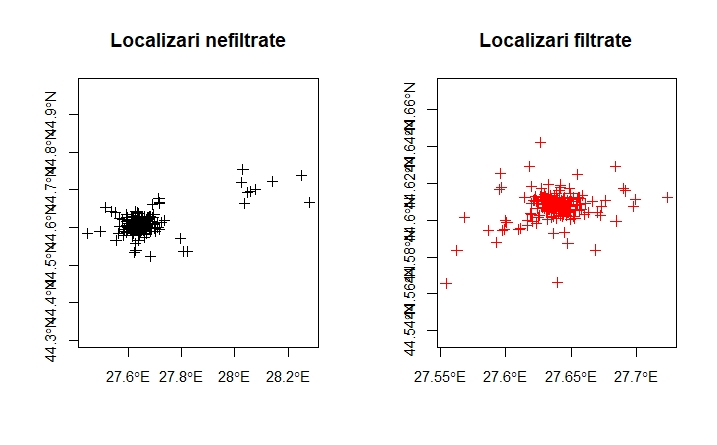
\includegraphics[width=\textwidth]{Fig12.jpeg}
\caption{Distribuția spațială a localizărilor neprelucrate și prelucrate cu filtru de viteză.} \label{fig12}
\end{figure}

\section{Pachete software pentru prelucrare avansată a datelor}
\paragraph{Movebank}
Movebank este o bază de date online în care cercetătorii pot depozita datele de localizare privat sau public. Are facilități pentru recepția automată a datelor Argos sau GPS, care pot fi vizualizate în timp real. De asemenea, pune la dispoziție facilități de filtrare a datelor, inclusiv filtrul Douglas-Argos. Seturile de date pot fi îmbogățite cu date ancilare cum ar fi DEM Aster\\
\url{https://www.movebank.org/ }

\paragraph{ArcMET pentru ArcMap (Movement Ecology Tools for ArcGIS)}
Este un pachet de unelte ArcGIS ce poate manipula fișiere geodatabase. Are funcții complexe (Filter, Range, UDTrajectory) dar necesită prelucrare inițială a mărcii temporale.\\
\url{http://www.movementecology.net}

\paragraph{adehabitat (Analysis of Habitat Selection by Animals)}
Este un pachet R cu funcții pentru analiza selecției de habitat și home range. A fost arhivat de autori, astfel că deși este larg utilizat va avea probleme de compatibilitate cu noile versiuni de R.\\
\url{https://www.rdocumentation.org/packages/adehabitat/versions/1.8.20}

\paragraph{crawl: Fit Continuous-Time Correlated Random Walk Models to Animal Movement Data}
Construiește modele temporal continue corelate random-walk cu marca temporală drept covarianță. Modelul calculează indicii statistici utilizând filtrul Kalman.\\
\url{https://CRAN.R-project.org/package=crawl}

\paragraph{bsam: Bayesian State-Space Models for Animal Movement}
Pachetul bsam calculează indici statistici pentru modele state-space Bayesiene via JAGS. Este realizat pentru date Argos. Mișcările animalelor sunt asociate statistic cu anumite  comportamente – deplasare țintită, mișcare rapidă, mișcare relativ indirectă, mișcare lentă.\\
\url{https://CRAN.R-project.org/package=bsam}

\paragraph{MoveHMM An R package for the analysis of animal movement data}
Constituie o variantă bsam pentru alte categorii de localizări, de exemplu GPS. Utilizează modele Markov ascunse.\\
\url{https://CRAN.R-project.org/package=moveHMM}

\paragraph{ctmm: Continuous-Time Movement Modeling}
Pachetul R ctmm poate rula cele mai importante modele continuu temporale. De asemenea poate fi utilizat pentru estimarea home range (UD, kernel, MCP etc.).\\
\url{https://CRAN.R-project.org/package=ctmm}

\paragraph{trip: Tools for the Analysis of Animal Track Data}
Pachetul trip include funcții pentru manipularea datelor de mișcare, inclusiv Argos. Poate detecta valorile aberante, duplicate, filtrează viteza și poate converti obiecte trip din pachetul R trip și ltraj din pachetul R adehabitat.\\
\url{https://CRAN.R-project.org/package=trip}

\paragraph{Animal Movement Tools (amt): R-Package for Managing Tracking Data and Conducting Habitat Selection Analyse}
Calculează statistică de mișcare (exemplu viteza medie), prelucrează datele brute pentru analiza selecției de habitat.\\
\url{https://CRAN.R-project.org/package=amt}

\paragraph{argosfilter: Argos locations filter}

Filtrează datele Argos (viteză, duplicate), fiind util mai ales pentru specii marine.\\
\url{https://www.rdocumentation.org/packages/argosfilter/versions/0.63} 

\paragraph{SDLfilter: Filtering Satellite-Derived Locations}
Filtrează datele Argos (viteză, duplicate) utilizând filtre simple. Are funcții de reprezentare cartografică simplă.\\
\url{https://CRAN.R-project.org/package=SDLfilter}

\paragraph{dplyr}
Poate manipula datele R pregătindu-le pentru lucrul cu pachetele descrise mai sus. Principalele funcții sunt mutate, select, filter, summarise, arrange.\\
\url{https://dplyr.tidyverse.org/}

\section{Literatură recomandată}

\paragraph{Sikes, R. S., Animal, C.,\& Use Committee of the American Society of, M. (2016). 2016 Guidelines of the American Society of Mammalogists for the use of wild mammals in research and education. Journal of Mammalogy, 97(3), 663-688. doi:10.1093/jmammal/gyw078}

Ghid profesional de reguli pentru capturarea și manipularea mamiferelor. Este axat pe regulile din Statele Unite ale Americii, dar poate fi extrapolat în Europa, fiind compatibil cu European Union Humane Trapping Standards.

\paragraph{Boitani, L., \& Fuller, T. (2000). Research techniques in animal ecology: controversies and consequences: Columbia University Press.}

O carte completă despre tehnici de cercetare în ecologia populațiilor, include informații detaliate despre conceptul de home range, estimatori de home range și selecție de habitat.

\paragraph{CLS. (2016). Argos User's Manual. Retrieved from http://www.argos-system.org/manual/}

Manualul de operare Argos CLS cuprinde toate detaliile tehnice ale sistemului, aduse la zi. În materialul de față au fost tratate cele mai importante probleme, dar tehnologia este în schimbare continuă, astfel că rămâne o resursă indispensabilă pentru interpretarea datelor obținute în teren.\\ 
Înainte de a decide utilizarea tehnologiei Argos citiți cu atenție manualul CLS și ghidul realizat de noi și puneți întrebări consultantului despre aspectele tehnice neclare. Argos este o tehnologie deosebit de utilă pentru foarte multe specii, dar, după cum am arătat și în acest ghid, localizările nu sunt de precizie GPS și sistemul are limitări care trebuie luate în considerare când se prelucrează și interpretează datele.

\paragraph{Silvy, N. J. (2012). The Wildlife Techniques Manual: Volume 1: Research. Volume 2: Management 2-vol. Set: The Johns Hopkins University Press.}

O altă sursă importantă de informații despre tehnicile de monitorizare a animalelor sălbatice, utilă mai ales pentru explicațiile și literatura despre capturare. Include informații foarte utile despre metode de tranchilizare.

\paragraph{White, G. C., \& Garrott, R. A. (2012). Analysis of wildlife radio-tracking data: Elsevier.}

O carte mai veche, din anii 1990,  retipărită în anul 2012, utilă pentru înțelegerea conceptelor de bază din ecologia mișcărilor animalelor (home-range, selecția de resurse).

\paragraph{Hooten, M. B., Johnson, D. S., McClintock, B. T., \& Morales, J. M. (2017). Animal movement: statistical models for telemetry data: CRC Press.}

Cartea descrie pe larg toate metodele moderne de analiză statistică a datelor de telemetrie. Abordarea este una practică, modelele fiind demonstrate cu exemple ce pot fi reproduse. Practic, cartea oferă o perspectivă completă a acestui domeniu și poate ghida cercetătorul către metoda potrivită de analiză.

\paragraph{Wickham, H., \& Grolemund, G. (2016). R for data science: import, tidy, transform, visualize, and model data: O'Reilly.}

Cum majoritatea modelelor pot fi rulate în R cu pachete dedicate, R for data science poate fi folosită pentru a învăța metode simple de manipulare și curățare a datelor. În acest manual lucrăm cu dplyr, dar setul de pachete numit tidyverse oferă soluții la aproape orice problemă întâlnită în R. O investiție de timp în învățarea acestui pachet va oferi cercetătorului acces la toate metodele moderne de analiză în R. Cartea poate fi accesată gratuit http://r4ds.had.co.nz/

\paragraph{Pop IM, Bereczky L, Chiriac S, Iosif R, Nita A, Popescu VD, Rozylowicz L (2018) Data from: Movement ecology of brown bears (Ursus arctos) in the Romanian Eastern Carpathians. Dryad Digital Repository. https://doi.org/10.5061/dryad.jk127ng}

Deși nu este o carte și nici un set de unelte complet, scriptul elaborat în cadrul proiectului Biomovefix oferă un exemplu de cadru conceptual de analiză a datelor de localizare. Acoperă calcule de home-range, testarea ipotezelor, crearea graficelor.

\section{Mulțumiri}
Manualul a fost realizat în cadrul proiectului experimental demonstrativ \textbf{Aplicații Argos pentru monitorizarea în timp real a animalelor sălbatice în România, cod PN-III-P2-2.1-PED-2016-0568}, finanțat de \textbf{Unitatea Executivă pentru Finanțarea Învățământului Superior, a Cercetării, Dezvoltării și Inovării} (\url{www.uefiscdi.ro}).
\bibliographystyle{vancouver-compatible}
\bibliography{manual-argos.bib}

\end{document}
